% template adapted from https://github.com/jgm/pandoc-templates/blob/master/default.latex

%%% STYLE %%%
\documentclass[12pt,]{article}

%%% PACKAGES %%%

% fonts
\usepackage{lmodern}

% pdf
\usepackage{pdfpages}

% formulae
\usepackage{amssymb,amsmath}
\usepackage{ifxetex,ifluatex}
\usepackage{fixltx2e}
\usepackage[T1]{fontenc}
\usepackage[utf8]{inputenc}

% hyperlinks
\IfFileExists{upquote.sty}{\usepackage{upquote}}{}
\IfFileExists{microtype.sty}{%
\usepackage[]{microtype}
\UseMicrotypeSet[protrusion]{basicmath} % disable protrusion for tt fonts
}{}
\PassOptionsToPackage{hyphens}{url} % url is loaded by hyperref
\usepackage[unicode=true]{hyperref}
  \PassOptionsToPackage{usenames,dvipsnames}{color} % color is loaded by hyperref
\definecolor{maroon}{cmyk}{0, 0.87, 0.68, 0.32}
\hypersetup{
      colorlinks=true,
    linkcolor=maroon,
    citecolor=blue,
    urlcolor=blue,
      breaklinks=true}
\urlstyle{same} % don't use monospace font for urls

% geometry
\usepackage[left=2cm,right=2cm,top=2cm,bottom=2cm]{geometry}
\renewcommand{\baselinestretch}{1.1}

% Bibliography
\usepackage{natbib}
\bibliographystyle{plainnat}

% Tables
\usepackage{longtable,booktabs}
% Fix footnotes in tables (requires footnote package)
\IfFileExists{footnote.sty}{\usepackage{footnote}\makesavenoteenv{long table}}{}

% graphics
\usepackage{graphicx,grffile}
\makeatletter
\def\maxwidth{\ifdim\Gin@nat@width>\linewidth\linewidth\else\Gin@nat@width\fi}
\def\maxheight{\ifdim\Gin@nat@height>\textheight\textheight\else\Gin@nat@height\fi}
\makeatother
\setkeys{Gin}{width=\maxwidth,height=\maxheight,keepaspectratio}

% indent
\IfFileExists{parskip.sty}{%
\usepackage{parskip}
}{% else
\setlength{\parindent}{0pt}
\setlength{\parskip}{6pt plus 2pt minus 1pt}
}

% prevent overfull lines
\setlength{\emergencystretch}{3em}  
\providecommand{\tightlist}{%
\setlength{\itemsep}{0pt}\setlength{\parskip}{0pt}}

\setcounter{secnumdepth}{0}

% paragraphs
\usepackage{titlesec}
\let\oldsection\section
\renewcommand\section{\newpage\oldsection}
\titleformat{\section}
{\huge\center\scshape}{\thesection}{1em}{}[{\titlerule[0.8pt]}]
\titleformat*{\subsection}{\LARGE\bfseries}
\titleformat*{\subsubsection}{\Large\bfseries}
\titleformat*{\paragraph}{\large\bfseries\itshape}
\titleformat*{\subparagraph}{\normalsize\itshape}


% set default figure placement to htbp
\makeatletter 
\def\fps@figure{htbp}
\makeatother

%%% BODY %%%
\usepackage{amsthm}
\newtheorem{theorem}{Theorem}[section]
\newtheorem{lemma}{Lemma}[section]
\theoremstyle{definition}
\newtheorem{definition}{Definition}[section]
\newtheorem{corollary}{Corollary}[section]
\newtheorem{proposition}{Proposition}[section]
\theoremstyle{definition}
\newtheorem{example}{Example}[section]
\theoremstyle{remark}
\newtheorem*{remark}{Remark}
\begin{document}

% First pages
  % First page
  
\includegraphics{images/logos}
  
  \begin{center}
    \vspace*{\stretch{1}}
    \LARGE{\textbf{Mémoire de stage}} \\
    \vspace*{\fill}
    \large{présenté par} \\
    \large{Sylvain SCHMITT} \\
    \vspace*{\fill}
    \large{pour obtenir le diplôme national de master} \\
    \large{mention Biodiversité, écologie, évolution} \\
    \small{parcours Biodiversité végétale et gestion des écosystèmes tropicaux (BIOGET)} \\
    \vspace*{\fill}
    \large{Sujet :} \\
    \Large{\textbf{A COMPLETER}} \\
    \vspace*{\fill}
    \large{soutenu publiquement le XX.xxxx.201X} \\
    \large{à Kourou} \\
    \vspace*{\fill}
    \large{devant le jury suivant :} \\
    \vspace*{\fill}
    Dr Bruno HÉRAULT  \emph{Tuteur de stage} \\
    Titre Prénom NOM  \emph{Examinateur} \\
    Titre Prénom NOM  \emph{Examinateur} \\
    Dr Stéphane TRAISSAC  \emph{Enseignant-réferent} \\
    \vspace*{\stretch{1}}
  \end{center}
  
  % Second page
  \newpage
  \vspace*{\fill}
  \emph{Les opinions émises par les auteurs sont personnelles et n'engagent pas AgroParisTech.}
  \newpage

\tableofcontents

\section*{Résumé et Abstract}\label{resume-et-abstract}
\addcontentsline{toc}{section}{Résumé et Abstract}

Écrire le résumé français ici\ldots{}

Write the english abstract here\ldots{}

\section*{Acknowledgments}\label{acknowledgments}
\addcontentsline{toc}{section}{Acknowledgments}

I would like to thank\ldots{}

\begin{itemize}
\tightlist
\item
  Bruno
\item
  Stéphane
\item
  Laurent
\item
  Fabian
\item
  Isabelle
\item
  Jérôme
\item
  Camilla
\item
  Aurélie
\item
  Éric
\item
  \ldots{}
\end{itemize}

\section*{Introduction}\label{introduction}
\addcontentsline{toc}{section}{Introduction}

Sutainable forest management in the tropics (i.e.~managed selective
harvesting of timber) has been widely promoted internationnaly to combat
tropical deforestation and degradation \citep{Zimmerman2012}. Currently
tropical logging accounts for one eight of global timber production
\citep{Blaser2011} and is still increasing. Most tropical timber
production originates from selective logging, the targeted harvesting of
timber from commercial species in a single cuttint cycle
\citep{Martin2015}.

On the other hand, tropical rainforests have fascinated ecologists due
to their outstanding diversity \citep{connell_diversity_1978}.
Effectively tropical forests host over half of the Earth's biodiversity
\citep{Scheffers2012}. High biodiversity from tropical rainforests is
the source of many ecosystem functions. Amongst others, tropical forests
play a key role in biogeochemical cycles, including carbone storage
\citep{Lewis2004}. \textbf{Add insights into carbon storage role of
tropical forest.} Ecosystem functions from tropical forests support
numerous ecosystem services, such as timber production and climate
regulation.

But several authors argue that selective logging represents a major
threat to biodiversity
\citep{Carreno-Rocabado2012, DeAvila2015, Gibson2013, Martin2015, Zimmerman2012},
challenging the sustainable definition from current selective logging.
We consequently need to assess both short and long term impacts of
selective logging on tropical forest ecosystems to implement better
syslvicultural practives in order to reach sustainability.

The question of selective logging impact on tropical forest can be
directly related to the emerging field of biodiversity and ecosystem
functionning \citep{Loreau2000}. Tropical forest outstanding
biodiversity will be both a factor and a result of forest ecosystem
response to logging disturbance. And forest ecosystem response to
logging disturbance will directly modify ecosystem functionning in both
short and long term. Consequently assessing selective logging effect on
tropical forest linking biodiversity and ecosystem seems an obvious and
promising way \citep{Loreau2010}. \textbf{Paragraph to fully review !}

Negative short term impacts of selective logging have been assessed
\citetext{\citealp{Carreno-Rocabado2012}; \citealp{DeAvila2015}; \citealp[but
see][]{Martin2015}}. Much less is known about the long term impact
\citep{Osazuwa-Peters2015}. The main reason is the difficulty to conduct
long term empirical study \citep[but see][]{Herault2010}, which can be
completed by the use of forest simulators
\citep{Huth2004, Khler2004, Ruger2008, Tietjen2006}. Individual-based
models of forest dynamics present the perfect framework to develop such
joint biodiversity-ecosystem approaches \citep{Li}. Individual-based
models describe forest `patches' accumulating carbon through time,
assessing tree growth within the patch, or releasing carbon through gap
opening \citep{Bugmann2001}. Up to several dozens of different Plant
Functional Types (PFTs) are generally defined and models can sometimes
be fully spatially explicit \citep{Pacala1996}. Recently, the forest
growth simulator TROLL \citep{Chave1999}, an individual-based and
spatially explicit forest model, was developped to introduce recent
advances in plant physiological community. TROLL model relates
physiological processes to species-specific functional traits
\citep{Li}. Consequently, TROLL model allow to simulate fully a
neotropical forest biodiversity to study biodiversity-ecosystem
functionning link response to logging disturbance.

\textbf{Major question greater diversity (taxonomic and functional)
brought a better resilience to disturbance ?}

\section{Model description}\label{model-description}

\subsection{Overview}\label{overview}

TROLL model each tree indivdually in a located environment. Thus TROLL
model, alongside with SORTIE \citep{Pacala1996, Uriarte2009} and FORMIND
\citep{Fischer2016, Kohler1998}, can be defined as an individual-based
and spatially explicit forest growth model. TROLL simulates the life
cycle of individual trees from recruitment, with a diameter at breast
height (dbh) above 1 cm, to death with growth and seed production. Trees
are growing in a located light environment explicitly computed witin
voxels of 1 \(m^3\). Each tree is consistently defined by its age,
diameter at brest height (dbh), height (h), crown radius (CR), crown
depth (CD) and leaf area (LA) (see figure \ref{fig:TROLLtree}). Tree
geometry is calculated with allometric equations but leaf area vary
dinamically within each crown following carbon allocations. Voxels
resolution of 1 \(m^3\) allow the establishment of maximum one tree by
1x1 m pixels. Each tree is flagged with a species label inherited from
the parent tree through the seedling recruitment. A species label is
associated to a number of species specific parameters (see table
\ref{tab:traits}) related to functional trait values which can be
sampled on the field.

\begin{figure}[htbp]
\centering
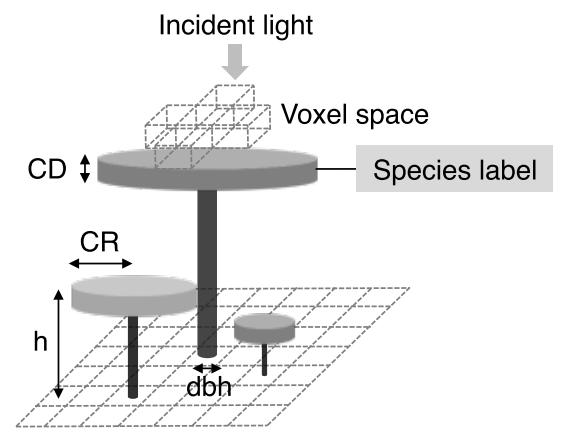
\includegraphics{images/TROLLtree.png}
\caption{\label{fig:TROLLtree}Individuals tree inside TROLL explicit spatial
grid from \citet{Li}. Tree geometry (crown radius CR, crown depth CD,
height h, diameter at breast height dbh) is updated at each timestep
following allometric relationship with assimilated carbon allocated to
growth. Each tree is flagged with a species label linking to its
species-specific attributes. Light is compputed explicitly at each
timestep for each voxel.}
\end{figure}

Carbon assimilation is computed over half-hourly period of a
representative day. Then allocation is computed to simulate tree growth
from an explicit carbone balance (in contrast to previous models).
Finally environment is updated at each timestep set to one month.
Seedlings are not simulated explicitly but as a pool. In addition
belowground processes, herbaceous plants, epiphytes and lianas are not
simulated inside TROLL. The source code is written in C++ and available
upon request. All modules of TROLL models are further detailed in
\protect\hyperlink{appendix-1-troll-model}{Appendix 1: TROLL model}.

\begin{longtable}[]{@{}lll@{}}
\caption{\label{tab:traits}Species-specific parameters used in TROLL from
\citet{Li}. Data originates from the BRIDGE \citep{Baraloto2010} and TRY
\citep{Kattge2011} datasets.}\tabularnewline
\toprule
Abbreviation & Description & Units\tabularnewline
\midrule
\endfirsthead
\toprule
Abbreviation & Description & Units\tabularnewline
\midrule
\endhead
\(LMA\) & leaf mass per area & \(g.m^{-2}\)\tabularnewline
\(N_m\) & leaf nitrogen content per dry mass &
\(mg.g^{-1}\)\tabularnewline
\(P_m\) & leaf phosphorous content per dry mass &
\(mg.g^{-1}\)\tabularnewline
\(wsg\) & wood specific gravity & \(g.cm^{-3}\)\tabularnewline
\(dbh_{thresh}\) & diameter at breasth height threshold &
\(m\)\tabularnewline
\(h_{lim}\) & asymptotic height & \(m\)\tabularnewline
\(a_h\) & parameter of the tree-height-dbh allometry &
\(m\)\tabularnewline
\bottomrule
\end{longtable}

Previous implementation of TROLL model used \citet{Reich1991a} allometry
to infer leaf lifespan \(LL\) from species leaf mass per area \(LMA\)
\citep[see \protect\hyperlink{appendix-1-troll-model}{Appendix 1: TROLL
model}]{Li}. But the use of the allometrie from \citet{Reich1991a} with
current implementation of the TROLL model resulted in an underestimation
of leaf lifespan for low LMA species. Consequently in the following
paragraph we suggest a new allometry.

Selective logging is defined as the targeted harvesting of timber from
species of interest. Consequently, tropical sylviculture can be
assimilated to a disturbance. The main difference between a disturbance
and selective logging is the targetting of both species and individuals
of interest. So we decided to first asses unselective disturbance effect
on tropical forest ecosystem to subsequently better understand selective
logging effect. First, we implemented a disturbance module inside TROLL
model to simulate unselective disturbance. Secondly, we implemented a
sylviculture module inside TROLL model to simulate selective logging in
regards to french Guiana practices.

\subsection{Leaf lifespan}\label{leaf-lifespan}

The underestimation of leaf lifespan for low LMA species with the
allometry from \citet{Reich1991a} resulted in indivduals unealistic
early death from carbon starvation. We gathered data from
TRY\citep{Kattge2011}, DRYAD \citep{chave_towards_2009} and GLOPNET
\citep{wright_worldwide_2004} datasets. We used an out of the bag method
applied on a random forest to select variables with highest importance
to explain leaf lifespan. We thus selected leaf mass per are \(LMA\),
leaf nitrogen content \(N\) and wood specific gravity \(wsg\). We then
used a bayesian approach to test different models with growing level of
complexity. The model with the best tradeoff between complexity (number
of parameters), convergence, likelihood, and prediction quality (root
mean square error of prediction RMSEP) was kept. We selected following
model with a maximum likelihood of 13.6 and a RMSEP of 12 months:

\begin{equation}
  LL_{d} \sim log\mathcal{N}({\beta_1}_d*LMA - {\beta_2}_d*N*\beta_3*wsg, \sigma)
  \label{eq:LL}
\end{equation}

Leaf lifespan \(LL\) follows a lognormal law with location infered from
leaf lifespan \(LMA\), nitrogen content \(N\) and wood specific gravity
\(wsg\) and a scale \(\sigma\). Each \({\beta_i}_d\) is following a
normal law located on \(\beta_i\) with a scale of \(\sigma_i\). All
\(\beta_i\), \(\sigma_i\), and \(\sigma\) are assumed without
presemption following a gamma law. \(d\) represents the dataset random
effects and encompass environmental and protocol variations (see
\protect\hyperlink{appendix-2-leaf-lifespan-model}{Appendix 2: Leaf
lifespan model} for more details).

\subsection{Disturbance}\label{disturbance}

Disturbance module was designed in the simplest way in order to relate
the ecosystem answer to volume lost without any individuals nor species
targetting. For a given iteration \(disturb_{iter}\), individuals are
picked randomly with a uniform law on the number of trees. Selected
individuals are then removed without trigerring a treefall to avoid any
side effect. The operation is repeated untill the disturbance result in
a defined lost basal area (\(disturb_{intensity}\) in \% of BA).

\subsection{Sylviculture}\label{sylviculture}

In french guiana context sylviculture can be narrow to selective
logging, which can be split in two steps: selection and harvesting.
Selection encompass choice of the havrestable area, tree designation by
the forest office, tree selection by the harvester, and removal off tree
probbed as rotten by the lumber. Harvesting encompass tree felling,
tracks opening, and long term damages (simplified in gap damages in
current TROLL implementation).

\subsubsection{Designation and
selection}\label{designation-and-selection}

One major limit of current implementation of TROLL model is that it
assumes a flat environment. Consequently the whole simulated area inside
TROLL is considered has an harvestable zone. With all commercial species
minimum and maximum harvestable diameter, TROLL calculates the total
harvestable volume \({V_h}_{tot}\). If the total harvestable volume
\({V_h}_{tot}\) exceed \(30~m^3.hectare^{-1}\), commercial species
minimum harvestable diameter \(dbh_{min}\) is increased untill
\({V_h}_{tot}\) is inferior to that upper limit.

In french guiana, tree harvesters are focusing on few species with
easier marketable wood, resulting in a tree harvest around
\(20~m^3.ha^{-1}\) (Laurent Descroix, ONF, personnal communication).
TROLL ranks each commercial species on its economic value, and randomly
remove individuals from lowest rank species untill it reaches total
harvested volume \({V_{hd}}_{tot}\) (\({V_{hd}}_{tot}\) was set to
\(25~m^3.hectare^{-1}\) in subsequent simulations).

\subsubsection{Rotten trees}\label{rotten-trees}

20 to 30 \% of designated trees are considered as rotten once probed by
the lumberman, and thus not harvested. Rotten trees are not random and
depends both on tree species and diameter. We gathered data from the
forest office (ONF, Laurent Descroix, personnal communication)
inventories precising if tree were probbed as rotten and their
corresponding species and diameter. In addition, tree plots and sawed
volume was informed. We then used a bayesian approach to model the link
between tree species and diameter and their risk to be probbed as rotten
by the lumberman. We test different models with growing level of
complexity and kept the model with the best tradeoff between complexity
(number of parameters), convergence, likelihood, and prediction quality
(root mean square error of prediction RMSEP):

\begin{equation}
  \begin{array}{c} 
    probbed~rotten \sim \mathcal{B}(P(probbed~rotten)) \\
    P(probbed~rotten) = logit^{-1}(\beta_0 + \beta_1*dbh) = \frac{e^{\beta_0 + \beta_1*dbh}}{1 + e^{\beta_0 + \beta_1*dbh}}
  \end{array}
  \label{eq:rotten}
\end{equation}

Tree \(probbed~rotten\) follows a \(Bernoulli\) law of probability
\(P(probbed~rotten)\). The odds for a tree to be probbed as rotten are
calculated with the sum of a base odd to be rotten \(\beta_0\) and a
diameter dependent odd calculated with \(\beta_1\). The probability for
a tree to be probbed as rotten \(P(probbed~rotten)\) is finally
calculated by taking the inverse logit \(logit^{-1}\) of the odd (see
\protect\hyperlink{appendix-3-rotten-tree-model}{Appendix 3: Rotten tree
model} for more details).

\subsubsection{Harvesting}\label{harvesting}

Due to crown aspects, treefall from logs are often random (whereas
difficult to manage, treefall can still be oriented, Laurent Descroix,
ONF, personnal communication). Consequently, TROLL consider treefall
from log as random like current natural treefall implementation inside
TROLL (see code {[}Appendix 1{]}).

Tree harvesting roads are split in three classes: truck roads, main
tractor track, and secondary track. Because TROLL assumes a flat
environment, the main track is opened starting from the middle of one
side of the simulated forest and untill it reaches the center with a
width of 6 meters. In most cases, secondary tracks are opened once trees
have been designated and the geolocation taken at a maximum distance of
30 meters from designated trees (Laurent Descroix, ONF, personnal
communication). To simulate secondary tracks, TROLL uses a loads map,
measuring every trees at a distance of 30 meters for each pixel, and a
track proximity maps of the closest existing track. Next, the model
select the pixel with the highest load and closest track, find the
closest existing track and join it by removing tree in the way with a
width of 5 meters. The operations are repeated untill no felt trees are
left.

\subsubsection{Gap damages}\label{gap-damages}

Most of models account long term damages due to selective logging with a
10 years increased mortality \citep{Huth2004, Khler2004, Ruger2008}. We
decided to model explicitly long term logging damages because of their
localised nature through a gap damages model. We gathered data from
Paracou dataset \citep{Guehl2004} in cenususes between 1988 and 1992 on
Paracou harvested plots. Individuals were categorized between alive,
dead, or recruited during the period. We measured each individual
distance to the closest gap. We then used a bayesian approach to test
the link between tree death in the four years following the log event
and distance to the closest gap. We adapted the model from
\citet{Herault2010} based on a disturbance index into:

\begin{equation}
  \begin{array}{c} 
    Death \sim \mathcal{B}(P(Death)) \\
    P(Death) = logit^{-1}(\theta + \beta*e^{\alpha*d_{gaps}}) = \frac{e^{\theta + \beta*e^{\alpha*d_{gaps}}}}{1 + e^{\theta + \beta*e^{\alpha*d_{gaps}}}}
  \end{array}
  \label{eq:death}
\end{equation}

\(Death\) of a tree follows a \(\mathcal{Bernoulli}\) law of probability
\(P(Death)\). The odds for a tree to die are calculated with the sum of
the natural tree death odd \(\theta\) and a perturbation index
\(\beta*e^{\alpha*d_{gaps}}\). The perturbation index depend on the
distance \(d_{gaps}\) of the tree \(i\) to the closest logging gap. The
probability for a tree to die \(P(Death)\) is finally calculated by
taking the inverse logit \(logit^{-1}\) of the odd.

\section{Material and Methods}\label{material-and-methods}

\subsection{Sensitivity analysis}\label{sensitivity-analysis}

\citet{Li} already assessed TROLL model sensitivity to several
parameters (\(k\) see \eqref{eq:PPFD}, \(\phi\) see \eqref{eq:LCP}, \(g1\)
see \eqref{eq:gs}, \(f_{wood}\) see \eqref{eq:DeltaV}, \(f_{canopy}\) see
\eqref{eq:DeltaLA} and \(m\) see \eqref{eq:db}) which they assumed having a
key role in model functioning. On the other hand, we decided to use
TROLL to study resistance and resilience of ecosystem face to
disturbance, highlighting the role of biodiversity. Consequently we
particulrarly needed to assess the importance of functional traits to
further better control and evaluate functional diversities. We also
needed to assess the sensitivity of TROLL model to the seed rain
constant (\(n_{ext}\), see \eqref{eq:next}) because we assumed it as one
of the main factors of tree recruitments after disturbance within
simulations.

TROLL model currenty uses leaf mass per area (\(LMA\) in \(g.m^{-2}\)),
leaf nitrogen content per dry mass (\(N_m\) in \(mg.g^{-1}\)), leaf
phosphorus content per dry mass (\(P_m\) in \(mg.g^{-1}\)), wood
specific gravity (\(wsg\) in \(g.cm^{-3}\)), diameter at breasth height
threshold (\(dbh_{thresh}\) in \(m\)), asymptotic height (\(h_{lim}\) in
\(m\)), and parameter of the tree-height-dbh allometry (\(a_h\) in
\(m\)). To assess the sensitivity of TROLL model to species functionnal
traits, we performed a sensitivity analysis by fixing species trait
values to their mean. Each trait was tested independently. We reduce to
a common mean traits with a Pearson's correlation value \(r \geq 0.8\)
(\(h_{max}\) and \(a_h\) with a correlation of \(r=0.98\)). To assess
the sensitivity of TROLL model to seed rain, we performed a sensitivity
analysis by fixing simulations seed rain constant to 2, 20, 200 and 2000
seeds per hectare.

Simulations were conducted on Intel Xeon(R) with 32 CPUs of 2.00GHz and
188.9 GB of memory. We assumed maturity of the forest after 500 years of
regeneration (Maréchaux \& Chave) and computed simulation 100 years
after a disturbance event with 40\% loss of basal area. Due to computer
limitations we did not run replicate (besides it should be necessary to
reduce simulation stochasticity). To assess ecosystem outputs
sensitivity to studied parameters, we compared it to 100 replicates of
control simulations with all parameters set to default values. Ecosystem
outputs outside of the range of the control replicates values are
significantly influenced by the studied parameter.

\subsection{Design of experiment}\label{design-of-experiment}

In order to assess the role of biodiversity in ecosystem answer to both
disturbance and sylviculture, we needed to create a space of experiments
encompassing both variation of disturbance, biodiversity and time.
Disturbance was represented by percentage of basal area loss (0\%, 25\%,
50\% and 75\%), or as a selective logging simulation. Biodiversity was
integrated with two components of its components: taxonomic and
functional diversities. We used species richness \(SR\) to represents
taxonomic diversity (5, 25, and 125 species). Functional diversity can
be related to numerous components, and \citet{Borgy2017} argued for 5:
richness, divergence, regularity, overlap and mean. Because mature
forest were created from a bare soil with TROLL simulations, we could
not control a priori divergence, regularity and overlap but only assess
theim before diturbance. Consequently, we focused on functional richness
with convex hull volume \(CHV\) and functional mean with community
weighted mean \(CWM\). For each level of species richness \(SR\), we
selected 20 communities with growing convex hull volume \(CHV\) but with
a community weighted means close to the regional species pool community
weighted means. Effectivelly, we did not wanted drastic change in
community means that could have more effect than functional richness
itself. This design of experiments resulted in 60 communities
(\(5~SR*20~CHV\)) and 240 simulations
(\(60 ~communities*4~levels~of~disturbance\)) over 600 years (maturity
being assumed after 500 years of regeneration \citep{Li}). Figure
\ref{fig:DOE} presents the design of experiment for communities
biodiversity after the mature forest were simulated, and thus before
disturbance. We obtained a broad range of both functionl dispersion
\(FDis\) and aboveground biomass \(AGB\) for simulated forest ecosystems
before disturbance.

\begin{figure}[htbp]
\centering
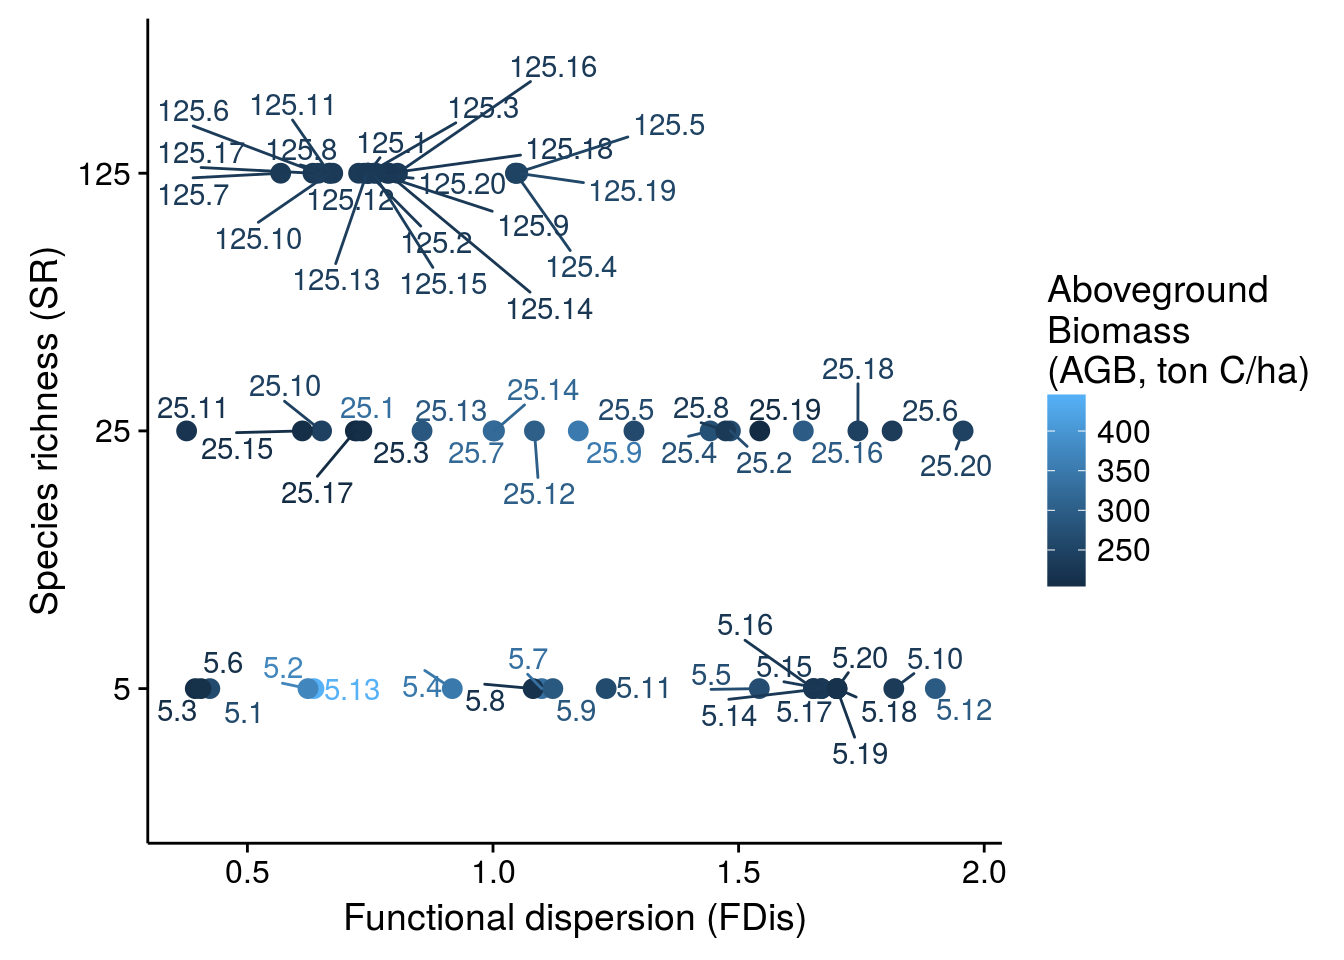
\includegraphics{master-thesis_files/figure-latex/DOE-1.pdf}
\caption{\label{fig:DOE}Experimental design before disturbance. Communities
are implemented along a gradient of species richness (SR) and functional
dispersion (FDis) resulting in a broad range of aboveground biomass
(AGB). FDis was caluclated based on 4 functional traits (leaf mass per
area, wood specific gravity, maximum diameter, and maximum height).}
\end{figure}

\subsection{Ecosystem answer analysis}\label{ecosystem-answer-analysis}

\subsubsection{Ecosystem functions}\label{ecosystem-functions}

Tropical forest ecosystems provides numerous ecosystem services linked
to several ecosystem functions. We decided to describe simiulated
tropical forests in two major functions: forest dynamic and forest
production. Forest dynamic was represented by aboveground biomass
(\(AGB\) in \(ton~C.ha^{-1}\)), basal area (\(BA\) in \(m^2.ha^{-1}\)),
total number of stem (\(N\)), number of stem above \(10~cm\) diameter
(\(N10\)), and number of stem above \(30~cm\) diameter (\(N30\)). Forest
production was represented by growth pimary productivity (\(GPP\) in
\(MgC.ha^{-1}\)), net pimary productivity (\(NPP\) in \(MgC.ha^{-1}\)),
tree autotrophic respiration in day (\(Rday\) in \(MgC.ha^{-1}\)) and
tree autotrophic respiration in night (\(Rnight\) in \(MgC.ha^{-1}\)).

The resilience of metrics values post disturbance were assessed through
\citet{Henry2012} formula:

\begin{equation}
  R\left(t\right)=\frac{Recovery\left(t\right)}{Loss\left(t_d\right)} \approx \frac{X_T(t)}{X_C(t)}
  \label{eq:Resilience}
\end{equation}

The resilience of the system \(R(t)\) at the time \(t\) is described by
the ratio of recovery \(Recovery(t)\) at time \(t\) to loss suffered
\(Loss(t_d)\) at disturbance time \(t_d\). But in our peculiar case of
tropical forest ecosystems, the equilibrium used to calculate
\(Loss(t_d)\) can not be reduced to a specific time if the equilibrium
is dynamic. Consequently, to encompass undisturbed ecosystem variations
throught time, we simulated an undisturbed control ecosystem \(C\). And
the resilience of the system \(R(t)\) at the time \(t\) was defined as
the ratio of the ecosystem metric values in the disturbed simulation
\(X_T(t)\) over the the ecosystem metric values from the control
\(X_C(t)\) . Thus, the value of resilience \(R(t)\) is normalized for
all simulations and metrics. \(R(t)\) will be equal to \(R_{eq} = 1\)
when reaching the equilibrium value. Consequently we can calculate an
euclidean distance to equilibrium \(d_{eq}(t)\) as
\(d_{eq}(t) = \sqrt{(R_{eq} - R(t))^2}\). Ecosystem euclidean distance
to equilibrium was calculated in a multi-dimensional space for the two
functions described above: forest dynamic (AGB, BA, N, N10, and N30) and
forest production (GPP, NPP, Rday, and Rnight). We then used cummulative
integral over time of eulcidean distance to equilibrium to assess
simulations resilience.

\subsubsection{Biodiversity effect}\label{biodiversity-effect}

Biodiversity is not only a facet of the experimental design and an
ecosystem output through forest diversity, but also interact on
ecosystem functioning and consequently on its answer to disturbance.
Biodiversity ecosystem functioning relation can be split in
complementarity and selection effect with \citet{Loreau2001}
partitioning:

\begin{equation}
  \begin{array}{c}
    NE = X_O - X_E = CE + SE \\
    CE = N* \overline{\Delta RX} \overline{M}\\
    SE = N*cov(\Delta RX,M)
  \end{array}
  \label{eq:BiodivPart}
\end{equation}

Biodiversity net effect \(NE\) is based on the difference between
ecosystem variable \(X\) observed value \(X_O\) within the community
mixture of species and its expected value \(X_E\) if species performance
were equal to their performance in monocultures. This effect can be
partitioned between complementarity effect \(CE\), representing niche
partitionning, positive interactions, and resource supply, and selectvie
effect \(SE\) due to dominant species pool driving the ecosystem. Both
metrics depend on the variation of relative ecosystem variable
\(\Delta RX\):

\begin{equation}
  \Delta RX_{sp} = \frac{X_{sp}(mixture)}{X_{sp}(monoculture)} - P_{sp}
  \label{eq:DeltaRY}
\end{equation}

\(X_{sp}\) is the ecosystem variable value for one species either in
mixture \(X_{sp}(mixture)\) or in monoculture \(X_{sp}(monoculture)\).
\(P_{sp}\) is the proportion of the species in the mixture represented
by species relative abundance. Consequently, \(CE\) averages diversity
effects of all species presents in the mixture (both negatives and
positives). Whereas \(SE\) become positive when dominant species
outperform theimselves in mixture than in monoculture, and negative when
less dominant species outperform theimselves in mixture than in
monoculture \citep{Tobner2016}. But similarly to resilience measurement,
biodiversity net effect \(NE\) can be in a dynamic equilibrium and vary
over time without disturbance. So in order to correctly assess selection
and complementarity effect in answer to disturbance, we normalized it by
undisturbed control ecosystem net effect \(NE_C\) to measure treatments
net effect resilience \(R(NE_T)\):

\begin{equation}
  R(NE_T) = \frac{NE_T}{NE_C} = \frac{SE_T}{NE_C} + \frac{CE_T}{NE_C}
  \label{eq:RNE}
\end{equation}

Resilience trajectories of ecosystem variable after disturbance were
partitioned between complementarity effect \(CE\) and selection effect
\(SE\). In order to do that, the design of experiment was repeated for
each species indivdually representing 652 simulations of monoculture.

\section{Results}\label{results}

\subsection{Sensitivity}\label{sensitivity}

\subsection{Disturbance}\label{disturbance-1}

\subsubsection{Ecosystem functions}\label{ecosystem-functions-1}

We transformed all ecosystem outputs from the 240 disturbance
simulations in resilience metrics normalizing the treatment values by
their corresponding control (Figure \ref{fig:datatrans} A et B). We then
gathered ecosystem outputs by main ecosystem functions (forest dynamic,
forest production and forest diversity) to compute ecosystem distance to
equilibrium (Figure \ref{fig:datatrans} C). Finally, we integrated
distance to equilibrium in a cummulative sum over time (Figure
\ref{fig:datatrans} D).

\begin{figure}[htbp]
\centering
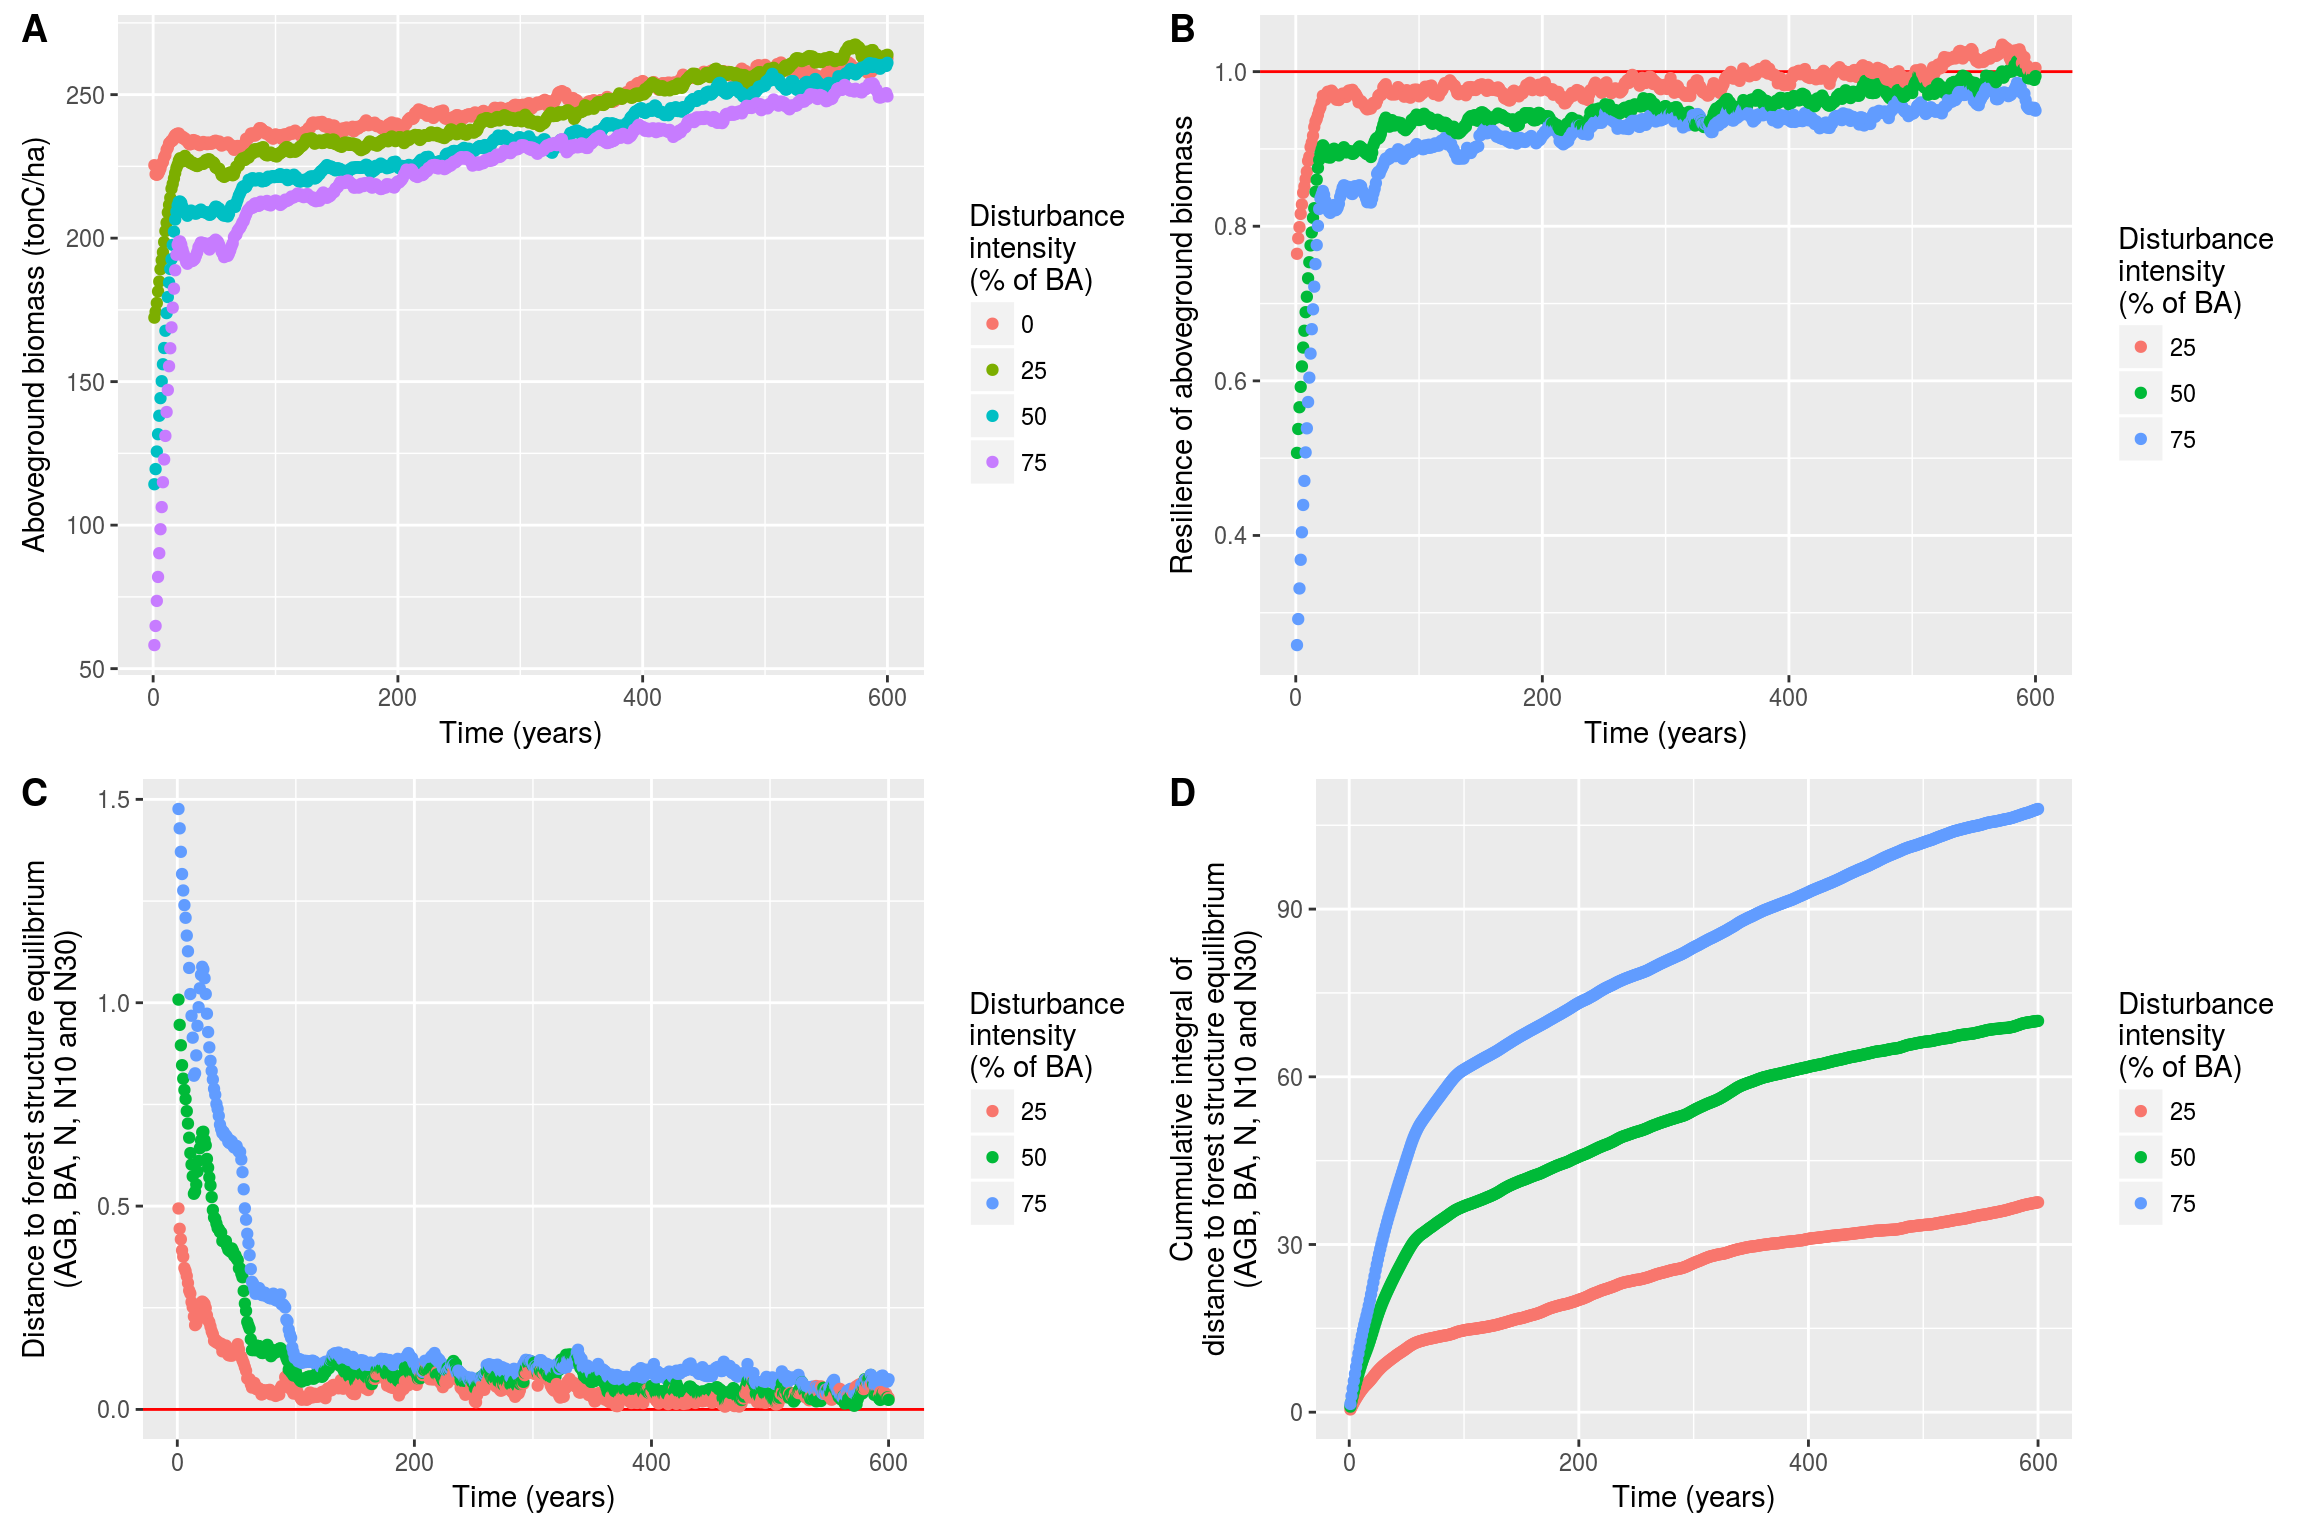
\includegraphics{master-thesis_files/figure-latex/datatrans-1.pdf}
\caption{\label{fig:datatrans}Ecosystem outputs data transformation.
Ecosystem outputs (\textbf{A}) are normalized by the control value over
time to calculate resilience (\textbf{B}); resilience of different
ecosystem outputs is then used in a multidimensional space to caluclate
ecosystem distance to equilibrium (\textbf{C}); finally distance ot
equilibirum is integrated over time in a cummulative sum (\textbf{D}).}
\end{figure}

The ranking was stable over time for the 240 simulations. So we used the
cummulative integral after 600 years \(Ieq_{600}\) as a measurement of
ecosystem resilience. We compared cummulative integral after 600 years
to communities taxonomic and functional diversity for each leavel of
disturbance (see Figure \ref{fig:gIeq}). We found that increased
functional diversity \citep[FDiv,][]{villeger_new_2008} was reducing
cummulative integral from ecosystem distance to forest dynamic
equilibrium after 600 years (\(Ieq_{600}\)). In addition, functional
eveness was complementary reducing \(Ieq_{600}\). Finally species
richness was not directly link to \(Ieq_{600}\). Effectivelly, low
species richness could result in variant \(Ieq_{600}\), but increased
species richness resulted in increased functional diversity and
consequently lower \(Ieq_{600}\). We found similar results for all
disturbance levels and other ecosystem functions (forest production and
forest diversity, see
\protect\hyperlink{appendix-5-disturbance-simulations}{Appendix 5:
Disturbance simulations}).

\begin{figure}[htbp]
\centering
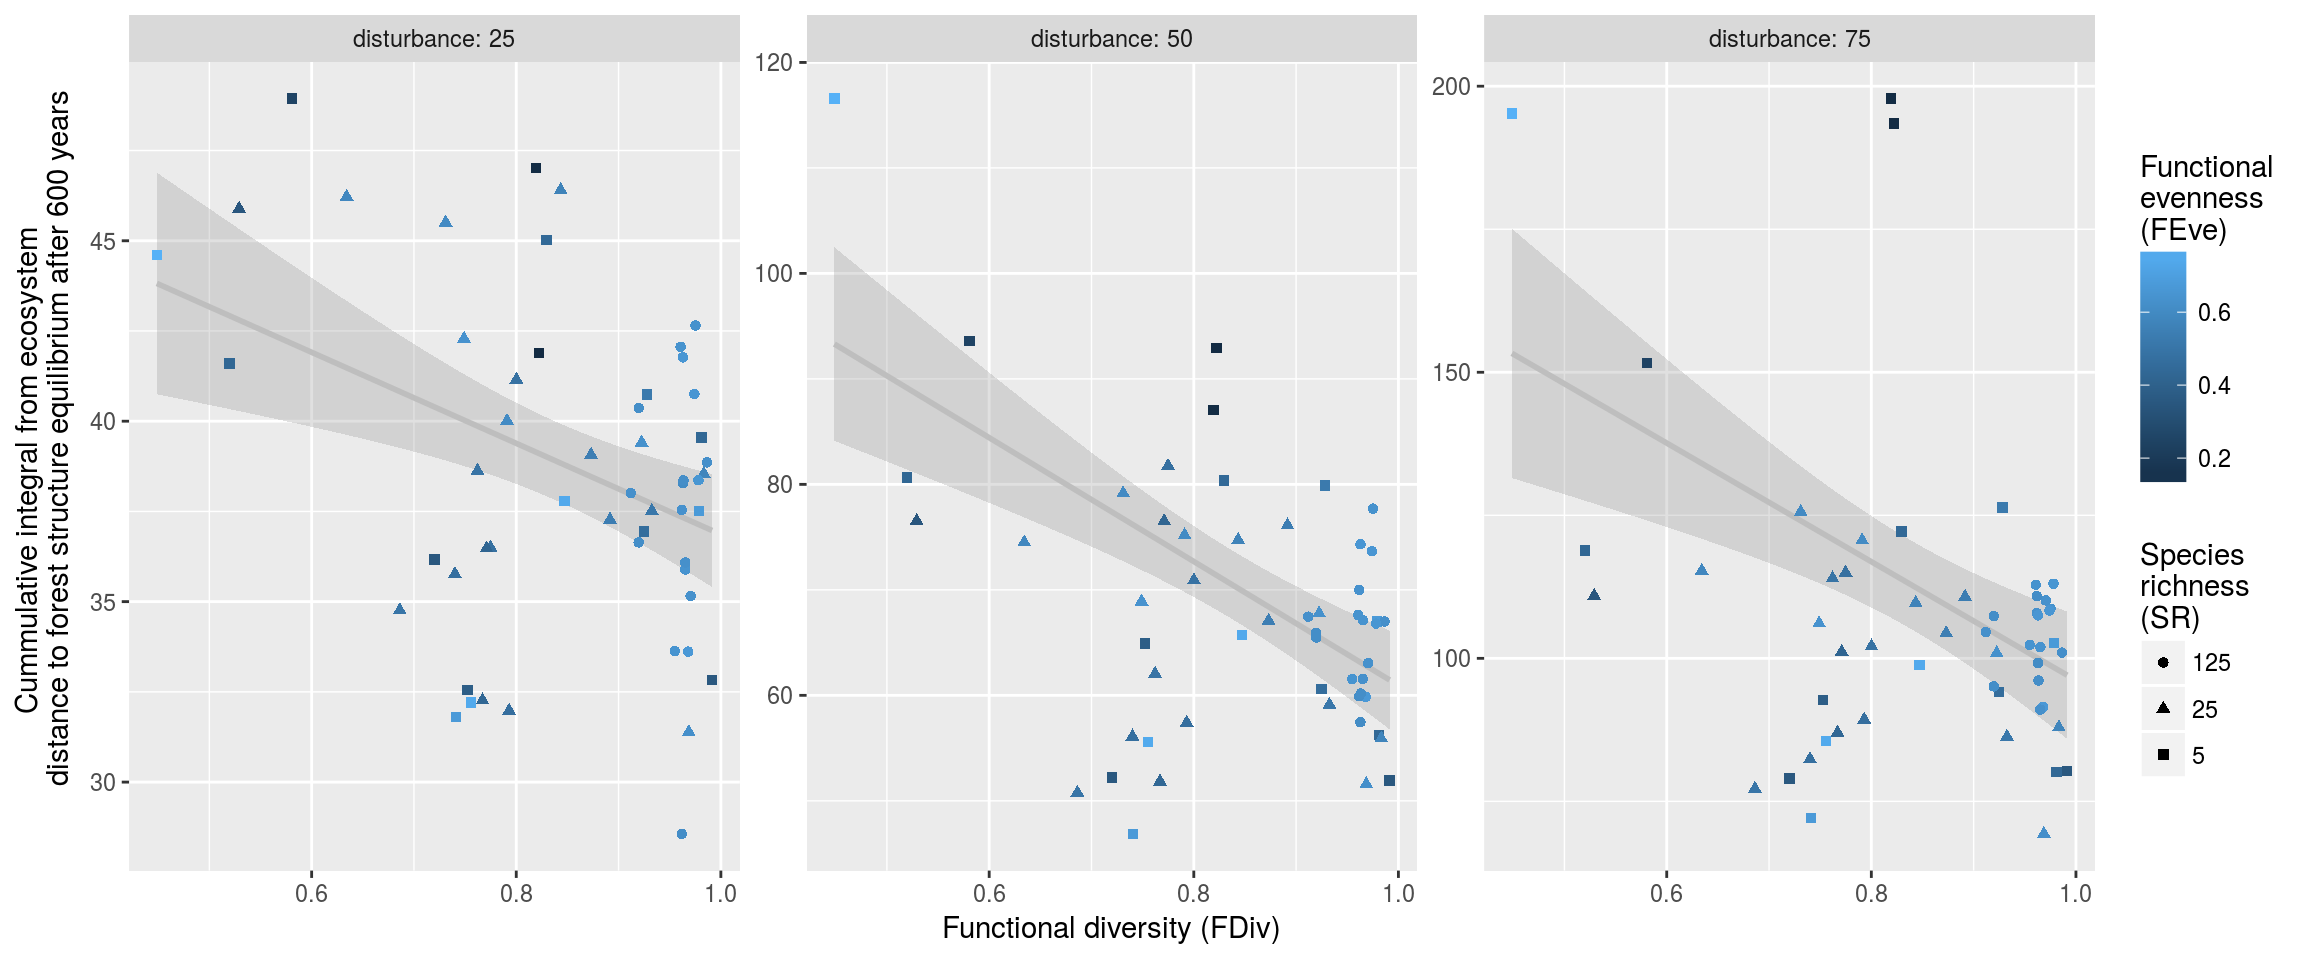
\includegraphics{master-thesis_files/figure-latex/gIeq-1.pdf}
\caption{\label{fig:gIeq}Ecosystem resilience after 600 years with taxonomic
and functional diversity for different levels of disturbance.
Cummulative integral from ecosystem distance to forest dynamic
equilibrium after 600 years was represented against functional diversity
\citep[FDiv,][]{villeger_new_2008} for different level of disturbance
(25, 50 and 75\% of total basal area); dot shapes represents the species
richness whereas dot color represents functional eveness
\citep[FEve,][]{villeger_new_2008}.}
\end{figure}

\subsubsection{Biodiversity effect}\label{biodiversity-effect-1}

We measured all ecosystem outputs biodiversity net effect in disturbance
simulations by comparing theim to their species corresponding
monoculture simulations. The net effect was then partition between
selection and complementarity effect. We normalized treatments effect by
control net effect (see Table \ref{tab:tNE}) to measure their
aboveground biomass resilience to disturbance (see Figure
\ref{fig:gBE}). We found that complementarity effect was recovering net
effect in the first decades untill it disappeared after a century. On
the contrary selection effect was reduced or even removed by the
disturbance. It increased during the whole simulation and was greater
than complementarity effect only after decades. The time lag for which
complementarity effect was non null and greater than selection effect
was increasing with disturbance intensity. Finally 600 years after the
disturbance event biodiversity net effect was still not recovered for a
disturbance intensity greater than 25\% of basal area. We obtained those
results for aboveground biomass. We found similar results but with an
amlified signal for basal area (\(BA\)) and stem abundance (\(N\) but
with an inverted signal because of the forest self thinning) (see
\protect\hyperlink{appendix-5-disturbance-simulations}{Appendix 5:
Disturbance simulations}). Finally, forest growth primary productivity
(\(GPP\)) recovered in few years (proportionnaly to disturbance), and
its net effect was maintained by complementarity effect (see
\protect\hyperlink{appendix-5-disturbance-simulations}{Appendix 5:
Disturbance simulations}).

\begin{longtable}[]{@{}lrrll@{}}
\caption{\label{tab:tNE}Table 1: Biodiversity net effect mean value and
standard deviation for different ecosystem variable.}\tabularnewline
\toprule
variable & mean & standard deviation & name & unit\tabularnewline
\midrule
\endfirsthead
\toprule
variable & mean & standard deviation & name & unit\tabularnewline
\midrule
\endhead
agb & 32.721 & 17.839 & aboveground biomass &
\(tonC.ha^{-1}\)\tabularnewline
ba & 1.633 & 0.743 & basal area & \(m^2.ha^{-1}\)\tabularnewline
n & 103.880 & 231.623 & number of stems & \(n.ha^{-1}\)\tabularnewline
n10 & -6.815 & 13.003 & number of stems above 10cm dbh &
\(n.ha^{-1}\)\tabularnewline
gpp & 0.147 & 0.047 & growth primary production &
\(MgC.ha^{-1}\)\tabularnewline
npp & -0.041 & 0.036 & net primary production &
\(MgC.ha^{-1}\)\tabularnewline
Rday & 0.046 & 0.018 & autotrophic respiration during day &
\(MgC.ha^{-1}\)\tabularnewline
Rnight & 0.074 & 0.030 & autotrophic respiration during night &
\(MgC.ha^{-1}\)\tabularnewline
\bottomrule
\end{longtable}

\begin{figure}[htbp]
\centering
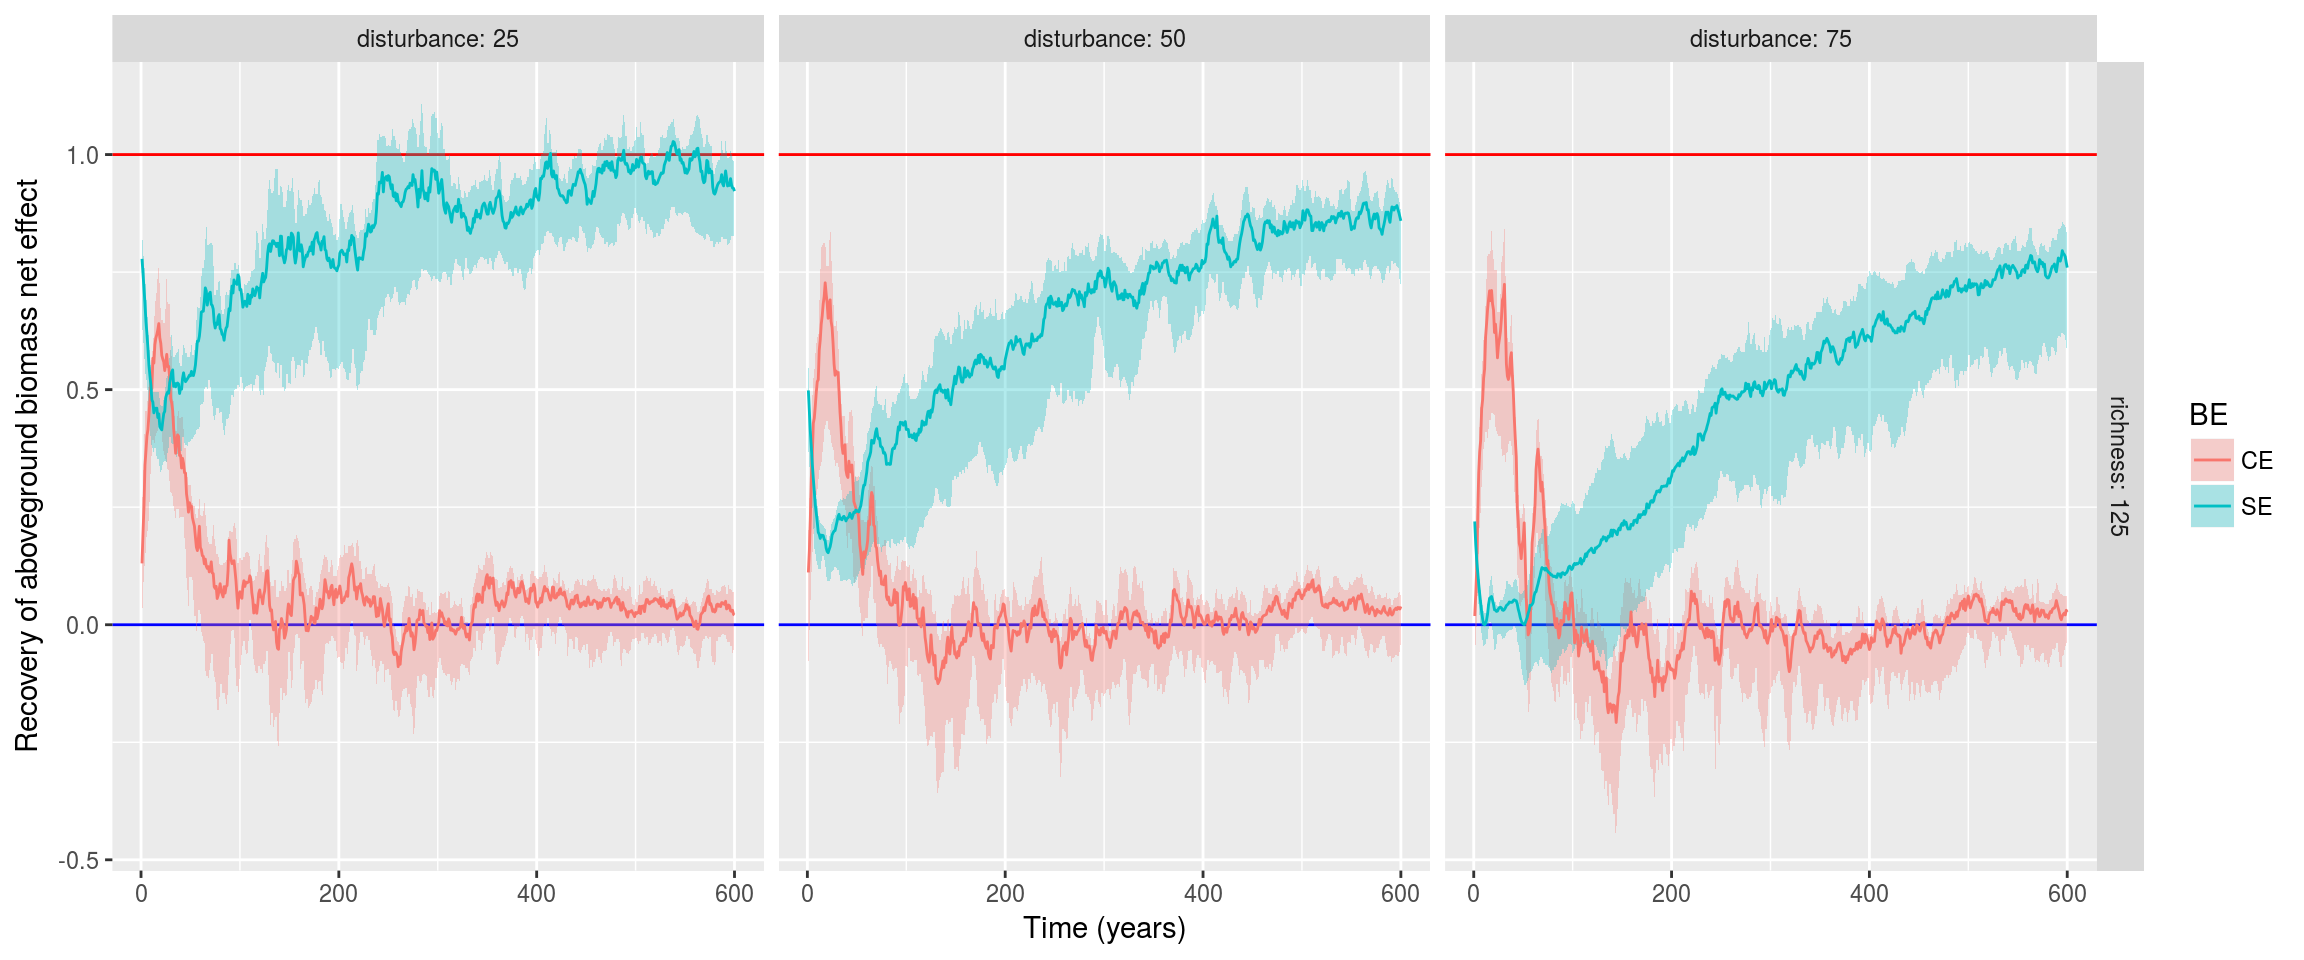
\includegraphics{master-thesis_files/figure-latex/gBE-1.pdf}
\caption{\label{fig:gBE}Resilience of complementarity and selection effects.
Complementarity effect (CE) and selection effect (SE) where normalized
by control net effect (NEc), thus measuring their resilience over time.}
\end{figure}

\subsection{Sylviculture}\label{sylviculture-1}

\section{Discussion}\label{discussion}

\appendix


\hypertarget{appendix-1-troll-model}{\section{Appendix 1: TROLL
model}\label{appendix-1-troll-model}}

I this Appendix we further detail modules of TROLL model.

\subsection{Abiotic environment}\label{abiotic-environment}

A voxel space, with a resolution of 1 \(m^3\), is used to explicilty
model the abiotic environment. For each tree crown, leaf area density is
calculated on tree geometry assuming a uniform distriution across voxels
occupied by the crown. Leaf area density is computed within each voxel
summing all tree crowns inside the voxel \(v\), and is denoted
\(LAD(v)\) (leaf area per voxel in \(m².m^{-3}\)). The vertical sum of
\(LAD\) from voxel \(v\) to the ground level defines \(LAI(v)\) (leaf
area per fround area in \(m^2.m^{-2}\) commonly called leaf area index):

\begin{equation}
  LAI(v) = \sum _{v'=v} ^\infty LAD(v') 
  \label{eq:LAI}
\end{equation}

Daily variations in light intensity (photosynthetic photon flux density
PPFD in \(\mu mol_{photons}.m^{-2}.s^{-1}\)), temperature (T in degrees
Celsius), and vapor pressure deficit (VPD in \(kPA\)) are computed to
assess carbon assimilation within each voxel of the canopy and for a
representative day per month (see Appendix 1 from \citet{Li} for further
details). Variation of PPFD Within the canopy is calculated as a loacal
Beer-Lambert extinction law:

\begin{equation}
  PPFD_{max,month}(v) = PPFD_{top,max,month}*e^{-k*LAI(v)}
  \label{eq:PPFD}
\end{equation}

The daily maximum incident PPFD at the top of canopy
\(PPFD_{top,max,month}\) is given as input. The extinction rate \(k\) is
assumed as constant, besides is variation with zenith angle and species
leaf inclination angle \citep{Meir2000}. Moreover only vertical light
diffusion is considered ignoring lateral light diffusion, which can have
an important role especially in logging gaps. Finally, intra-day
variation at half hour time steps \(t\) for a representative day every
month are used to compute \(PPFD_{month}(v,t)\), \(T_{month}(v,t)\) and
\(VPD_{month}(v,t)\). Water and nutrient process both in soil and inside
trees are not simulated.

\subsection{Photosynthesis}\label{photosynthesis}

\subsubsection{Theory}\label{theory}

Troll simulates the carbon uptake of each individual with the Farquhar,
von Caemmerer and Berry model of C3 photosynthesis \citep{Farquhar1980}.
Gross carbon assimilation rate (\(A\) in
\(\mu mol~CO_2. m^{-2}.s^{-1}\)) will be the minimum of eiter Rubisco
activity (\(A_v\)) or RuBP generation (\(A_j\)):

\begin{equation}
  A=min(A_v, A_j)~|~A_v=V_{cmax}*\frac{c_i-\Gamma^*}{c_i+K_m}~;~A_j=\frac{J}{4}*\frac{c_i-\Gamma^*}{c_i+2*\Gamma^*}
  \label{eq:A}
\end{equation}

\(V_{cmax}\) is the maximum rate of carboxylation
(\(\mu mol~CO_2.m^{-2}.s^{-1}\)). \(c_i\) is the \(CO_2\) partial
pressure at carboxylation sites. \(\Gamma^*\) is the \(CO_2\)
compensation point in absence of dark respiration. \(K_m\) is the
apparent knietic constant of the Rubisco. And \(J\) is the electron
transport rate (\(\mu mol e^-.m^{-2}.s^{-1}\)). \(J\) depends on the
light intensity with \(PPFD\):

\begin{equation}
  J = \frac{1}{2*\theta}*[\alpha*PPFD+J_{max}-\sqrt{(\alpha*PPFD+J_{max})^2}-4*\theta*\alpha*PPFD*J_{max}]
  \label{eq:J}
\end{equation}

\(J_{max}\) is the maximal electron transport capacity
(\(\mu mol e^-.m^{-2}.s^{-1}\)). \(\theta\) is the curvature factor. And
\(\alpha\) is the apparent quantum yield to electron transport
(\(mole^-.mol~photons^{-1}\)).

Carbon assimilation by photosynthesis will then be limited by the
\(CO_2\) partial pressure at carboxylation sites. Stomata controls the
gas concentration at carboxylation sites throught stomatal transport:

\begin{equation}
  A = g_s*(c_a-c_i)
  \label{eq:Ag}
\end{equation}

\(g_s\) is the stomatal conductance to \(CO_2\)
(\(molCO_2.m^{-2}.s^{-1}\)). TROLL simulates stomatal conductance
\(g_s\) with the model from \citep{Medlyn2011}:

\begin{equation}
  g_s = g_0 + (1 + \frac{g_1}{\sqrt{VPD}})*\frac{A}{c_a}
  \label{eq:gs}
\end{equation}

\(g_0\) and \(g_1\) are parameters from the model. TROLL model assume
\(g_0 \approx 0\) (empirically tested and considered as reasonable).

\subsubsection{Parametrization}\label{parametrization}

Leaf traits can be used as proxy of photosynthesis, especially leaf
nutrient content which directly play a role in it
\citep{wright_worldwide_2004}. \citet{Domingues2010} suggested that
\(V_{cmac}\) and \(J_{max}\) were both limited by the leaf concentration
of nitrogen \(N\) and phosphorus \(P\) (\(mg.g^{-1}\)):

\begin{equation}
  log_{10} V_{cmax-M} = min( 
  \begin{array}{c} 
    -1.56+0.43*log_{10} N-0.37*log_{10} LMA \\
    -0.80+0.45*log_{10} P-0.25*log_{10} LMA 
  \end{array} 
  )
  \label{eq:VcmaxM}
\end{equation}

\begin{equation}
  log_{10} J_{max-M} = min(
  \begin{array}{c} 
    -1.50+0.41*log_{10} N-0.45*log_{10} LMA \\
    -0.74+0.44*log_{10} P-0.32*log_{10} LMA 
  \end{array}
  )
  \label{eq:JmaxM}
\end{equation}

\(V_{cmax-M}\) and \(J_{max-M}\) are the photosynthetic capacities at
\(25^\circ C\) of mature leaves per leaf dry mass (resp.
\(\mu mol CO_2.g^-1.s^{-1}\) and \(\mu mol e^-.g^{-1}.s^{-1}\)). \(LMA\)
is the leaf mass per are (\(g.cm^{-2}\)). \(V_{cmax}\) and \(J_{max}\)
are calculated by multiplying \(V_{cmax-M}\) and \(J_{max-M}\) by
\(LMA\). \(V_{cmax}\) and \(J_{max}\) variation with temperature are
caluclated with \citet{Bernacchi2003} (see Appendix 2 from \citet{Li}
for further details).

TROLL computes leaf carbon assimilation \(A_l\) combining equations from
\eqref{eq:A} to \eqref{eq:JmaxM} for each tree crown voxel within in each
crown layer \(l\):

\begin{equation}
  A_l = \frac{1}{n_v*t_M} * \sum_v  \sum^{t_M}_{t=1} A(PPFD_{month}(v,t),VPD_{month}(v,t),T_{month}(v,t))
  \label{eq:Al}
\end{equation}

\(PPFD_{month}(v,t)\), \(VPD_{month}(v,t)\) , and \(T_{month}(v,t)\) are
derived from microclimatic data. \(n_v\) is the number of voxels within
crown layer \(l\). And the sum is calculated over the \(t_M\)
half-hourly intervals \(t\) of a tipical day.

\subsection{Autotrophic respiration}\label{autotrophic-respiration}

A large fraction of plants carbon uptake is actually used for plant
maintenance and growth respiration. The autotrophic respiration can
represents up to 65\% of the gross primary productivity but varies
strongly among species, sites, and environnements.

TROLL uses \citet{Atkin2015} database of mature leaf dark respiration
and associated leaf traits to compute leaf maintenance respiration:

\begin{equation}
  R_{leaf-M} = 8.5431-0.1306*N-0.5670*P-0.0137*LMA+11.1*V_{cmax-M}+0.1876*N*P
  \label{eq:Rl}
\end{equation}

\(R_{leaf-M}\) si the dark respiration rate per leaf dry mass at a
temperaure of \(25^\circ C\) (\(nmolCO_2.g^{-1}.s^{-1}\)). The other
terms are in equations \eqref{eq:VcmaxM} and \eqref{eq:JmaxM}. TROLL assume
leaf respiration during day light to be 40\% of leaf dark respiration,
and computes total leaf respiration by accounting for the legnth of
daylight.

TROLL model stem respiration (\(R_{stem}\) in \(\mu molC.s^{-1}\)) with
a constant respiration rate per volume of sapwood:

\begin{equation}
  R_{stem} = 39.6*\pi*ST*(dbh-ST)*(h-CD)
  \label{eq:Rs}
\end{equation}

dbh, h, CD and ST are tree diameter at breast height, height, corwn
depth and sapwoond thickness, respectively (\(m\)). TROLL assumes
\(ST=0.04~m\) when \(dbh>30~cm\) and an increasing \(ST\) for lower
\(dbh\).

Finally, TROLL computes both fine root maintenance respiration, as half
of the leaf maintenance respiration. Whereas coarse root and branch
maintenance respiration is computed as half of the stem respiration. And
growth respiration (\(R_{growth}\)) is assumed to account for 25\% of
the gross primary productivity minus the sum of maintenance
respirations.

\subsection{Net carbon uptake}\label{net-carbon-uptake}

Net primary production of carbon for one individual \(NPP_{ind}\)
(\(gC\)) is computed by the balance between gross primary production
\(GPP_{ind}\) and respirations \(R\):

\begin{equation}
  NPP_{ind} = GPP_{ind} - R_{maintenance} - R_{growth}
  \label{eq:NPP}
\end{equation}

TROLL partitions individuals total leaf area \(LA\) into three pools for
different leaf age classes corresponding to different photosynthesis
efficiency (young, mature and old leaves with \(LA_{young}\),
\(LA_{mature}\), and \(LA_{old}\) respectivelly). Consequently we can
compute growth primary production for one individual as:

\begin{equation}
  GPP_{ind} = 189.3 * \Delta t * \sum _{l= \lfloor h-CD \rfloor +1} ^{\lfloor h \rfloor} [A_l] * (\frac{LA_{young}}{2} + LA_{mature} + \frac{LA_{old}}{2})
  \label{eq:GPP}
\end{equation}

h and CD are tree height and crown depth, repectivelly (\(m\)).
\(\lfloor x \rfloor\) is the rounding function. \(\Delta t\) is the
duration of a timestep (\(year\)).

Thus, TROLL can compute carbon allocation to wood into an increment of
stem volume \(\Delta V\) (\(m^3\)):

\begin{equation}
  \Delta V = 10^{-6} * \frac{f_{wood}*NPP_{ind}}{0.5*wsg}*Senesc(dbh)
  \label{eq:DeltaV}
\end{equation}

\(f_{wood}\) is the fixed fraction of NPP allocated to stem and
branches. \(wsg\) is the wood specific gravity (\(g.cm^{-3}\), see
\ref{tab:traits}). TROLL assume large trees less efficient to convert
NPP as growth by using a size-related growth decline with function
\(Senesc\) after a specific diameter at brest height threshold
\(dbh_{thresh}\):

\begin{equation}
  Senesc(dbh) = max(0;3-2*\frac{dbh}{dbh_{thresh}})
  \label{eq:Senesc}
\end{equation}

Finally, TROLL can compute carbon allocation to canopy with canopy NPP
fraction denoted \(f_{canopy}\) and decomposed into leaf, twig and fruit
production. Carbon allocation to leaf results in a new young leaf pool,
whereas other leaf pools are updated as follow:

\begin{equation}
  \begin{array}{c} \\
   \Delta LA_{young} = \frac{2*f_{leaves}*NPP_{ind}}{LMA}-\frac{LA_{young}}{\tau_{young}} \\
  \Delta LA_{mature} = \frac{LA_{young}}{\tau_{young}} - \frac{LA_{mature}}{\tau_{mature}}\\
  \Delta LA_{old} = \frac{LA_{mature}}{\tau_{mature}} - \frac{LA_{old}}{\tau_{old}}
  \end{array}
  \label{eq:DeltaLA}
\end{equation}

\(\tau_{young}\), \(\tau_{mature}\), and \(\tau_{old}\) are species
residence times in each leaf pools (\(years\)). The sum of residency
time thus defined the leaf lifespan
\(LL = \tau_{young} + \tau_{mature} + \tau_{old}\) (\(years\)).
\(\tau_{young}\) is set to one month and \(\tau_{mature}\) is set to a
third of leaf lifespan \(LL\). Belowground carbon allocation is not
simulated inside TROLL.

\subsection{Tree growth}\label{tree-growth}

Once the increment of stem volume \(\Delta V\) calculated with equation
\eqref{eq:DeltaV}, TROLL convert it into an increment of tree diameter at
breast height denoted \(\Delta dbh\). TROLL infer tree height from
\(dbh\) using a Michaelis-Menten equation:

\begin{equation}
  h = h_{lim}*\frac{dbh}{dbh + a_h}
  \label{eq:h}
\end{equation}

On the other hand, we have the trunk volume
\(V = C * \pi * (\frac{dbh}{2})^2*h\), thus:

\begin{equation}
  \begin{array}{c} \\
    \Delta V = C*\frac{1}{2}*\pi*h*dbh*\Delta dbh + C * \pi * (\frac{dbh}{2})^2*h \\
    \Delta V = V*\frac{\Delta dbh}{dbh}*(3-\frac{dbh}{dbh + ah})
  \end{array}
  \label{eq:Deltadbh}
\end{equation}

Next, TROLL used the new trunk dimension (\(dbh\) and \(h\)) to update
tree crown geometry using allometric equations \citep{Chave2005}:

\begin{equation}
  \begin{array}{c} \\
    CR = 0.80 + 10.47*dbh - 3.33*dbh^2\\
    CD = -0.48 + 0.26*h~;~CD = 0.13 + 0.17*h~(h<5~m)
  \end{array}
  \label{eq:C}
\end{equation}

Finally, TROLL computes the mean leaf density within the crown (\(LD\)
in \(m^2.m^{-3}\)) assuming a uniform distribution:

\begin{equation}
  LD = \frac{LA_{young}+LA_{mature}+LA_{old}}{\pi*CR^2*CD}
  \label{eq:LD}
\end{equation}

\subsection{Mortality}\label{mortality}

Mortality is partitioned in three factors inside TROLL: background death
\(d_b\), treefall death \(d_t\) and negative density dependent death
\(d_{NDD}\). Because density dependent death \(d_{NDD}\) is still in
development inside TROLL we did not used it, so we will not detail is
computation.

\citet{chave_towards_2009} advocated for a wood economics spectrum
opposing fast growing light wood species species with high risk of
mortality to slow growing dense wood species with reduced risk of
mortality. Hence, background mortality is derived from wood specific
gravity \(wsg\) inside TROLL:

\begin{equation}
  d_b = m*(1-\frac{wsg}{wsg_{lim}})+d_n
  \label{eq:db}
\end{equation}

\(m\) (\(events.year^{-1}\)) is the reference background death rate for
lighter wood species (pioneers). \(d_n\) represents death by
carbohydrates shortage. If the number of consecutive day with
\(NPP_{ind} < 0\) \eqref{eq:NPP} is superior to tree leaf lifespan \(d_n\)
is set to 1 and remains null in other cases.

Mortality by treefall inside TROLL depends on a specifric stochastic
threshold \(\theta\):

\begin{equation}
  \theta = h_{max}*(1-v_T*|\zeta|)
  \label{eq:theta}
\end{equation}

\(h_{max}\) is the maximal tree height. \(v_T\) is the variance term set
to 0.3. \(|\zeta|\) is the absolute value of a random centered and
scaled Gaussian. If the tree hieght \(h\) is superior to \(\theta\) then
the tree may fall with a probability \(1-\theta/h\) \citep{Chave1999}.
The treefall direction is random (drawn from a uniform law
(\(\mathcal{U}[0,2\pi]\)). All tree in the trajectory of the falling
tree will be hurted through a variable denoted \(hurt\), incremented by
fallen tree height \(h\). If a tree height is inferior than its \(hurt\)
values then it may die with a probability
\(1-\frac{1}{2}\frac{h}{hurt}\). \(hurt\) variable is reset to null at
each timestep (\(month\)).

\subsection{Recruitment}\label{recruitment}

Once the tree became fertile they will start to disperse seeds. TROLL
consider tree as fertile after a specific height threshold
\(h_{mature}\) \citep{Wright2005}:

\begin{equation}
  h_{mature} = -11.47+0.90*h_{max}
  \label{eq:hmature}
\end{equation}

But TROLL is not considering seed directly through a seedbank, instead
seed might be interpreted as a seedling recruitment opportunity. The
number of reproduction opportunities per mature tree is denoted \(n_s\)
and set to 10 for all species. This assumption originates from a
trade-off between seed number and seed size resulting in equivalent
survival and recruitment probability. All \(n_s\) events are dispersed
with a distance randomly drawn from a Gaussian distribution.
Additionally, TROLL model consider external seedrain through \(n_{ext}\)
events of seed immigration:

\begin{equation}
  n_{ext} = N_{tot}*f_{reg}*n_{ha}
  \label{eq:next}
\end{equation}

N\_\{tot\} is the external seedrain per hectare (number of reproduction
opportunities). \(f_{reg}\) is the species regional frequency.
\(n_{ha}\) is the simulated plot size in \(ha\).

Finally, a bank of seedlings to be recruited is defined for each pixel.
If the ground-level light reaches a species light compensation point
\(LCP\) the species will be recruited:

\begin{equation}
  LCP = \frac{R_{leaf}}{\phi}
  \label{eq:LCP}
\end{equation}

\(R_{leaf}\) is the leaf respiration for maintenance (see \eqref{eq:Rl}).
\(\phi\) is the quantum yield (\(\mu mol C.\mu mol~photon\)) set to
0.06. If several species reach their \(LCP\), one is picked at random.
Seedlings are recruited with following intial geometry:

\begin{equation}
  \begin{array}{c} \\
    dbh = \frac{a_h}{h_{max} - 1}\\
    h = 1~m\\
    CR = 0.5~m\\
    CD = 0.3~m\\
    LD = 0.8~m^2.^{-3}
  \end{array}
  \label{eq:C}
\end{equation}

\hypertarget{appendix-2-leaf-lifespan-model}{\section{Appendix 2: Leaf
lifespan model}\label{appendix-2-leaf-lifespan-model}}

TROLL model previous implementation encompass Reich's 1991 and 1997 and
Wright's 2004 allometries to estimate leaf lifespan with
\citep{Reich1991a, Reich1997, wright_worldwide_2004}. But we have shown
that Reich's allometries are underestimating leaf lifespan for low LMA
species. Moreover simulations estimated unrealistically low aboveground
biomass for low LMA species. We assumed Reich's allometries
underestimation of leaf lifespan for low LMA species being the source of
unrealistically low aboveground biomass inside TROLL simulations. We
decided to find a better allometry with \citet{wright_worldwide_2004}
GLOPNET dataset.

\subsection{Material and methods}\label{material-and-methods-1}

We compiled functional traits from GLOPNET
\citep{wright_worldwide_2004}, TRY \citep{Kattge2011}, and DRYAD
\citep{chave_towards_2009} databases (see \ref{tab:A2traits}). We kept
dataset given by GLOPNET as origin dataset for observations. Dataset
defined as origin corresponded to leaf lifespan (\(LL\)) and most of the
time to leaf mass per area (\(LMA\)) and leaf nitrogen content per leaf
dry mass (\(Nmass\)). We measured variable importance in functionnal
traits to explain leaf lifespan with out-of bag method applied on a
random forest. Then, we used a béayesian apporach to test different
models with growing level of complexity. We retained the model with the
best tradeoff between model complexity (number of parameters \(K\)),
convergence, likelihood, and prediction quality (root mean sqaure error
of prediciton \(RMSEP\)). We finally tested the new allometry obtained
with the selected model with TROLL simulations.

\begin{longtable}[]{@{}lllr@{}}
\caption{\label{tab:A2traits}Functional traits gathered with
TRY.}\tabularnewline
\toprule
Name & Trait & Unit & TRYcode\tabularnewline
\midrule
\endfirsthead
\toprule
Name & Trait & Unit & TRYcode\tabularnewline
\midrule
\endhead
LL & Leaf lifespan (longevity) & month & 12\tabularnewline
SLA & Leaf area per leaf dry mass (specific leaf area, SLA) &
\(m^2.kg^{-1}\) & 11\tabularnewline
N & Leaf nitrogen (N) content per leaf dry mass & \(mg.g^{-1}\) &
15\tabularnewline
P & Leaf phosphorus (P) content per leaf dry mass & \(mg.g^{-1}\) &
14\tabularnewline
wsg & Stem dry mass per stem fresh volume (stem specific density) &
\(mg.mm^{-3}\) & 4\tabularnewline
\bottomrule
\end{longtable}

\subsection{Results}\label{results-1}

Out of the bag method applied on a random forest highlighted the
importance of leaf nitrogen content per leaf dry mass (\(N_m\)) to model
leaf lifespan (see \ref{tab:A2OOB}). \(N_m\) importance was higher than
leaf mass per area (158 against 96 percent of mean square error
increase) which was used as a proxy for leaf lifespan in previous
models. Finally, wood specific gravity (\(wsg\)) add also a significant
importance in leaf lifespan estimation.

\begin{longtable}[]{@{}lrr@{}}
\caption{\label{tab:A2OOB}Variable importance calculated with out-of the bag
method applied on a random forest. First column represents the mean
decrease in mean square error (\%IncMSE) whereas second column
represents the total decrease in node impurities, measured by the Gini
Index (IncNodePurety). Leaf lifespan (LL) is taken in GLOPNET database
from \citet{wright_worldwide_2004}. Leaf mass per area (LMA), and leaf
nitrogen content (Nmass) are taken both in TRY
(\url{https://www.try-db.org}) and GLOPNET databases. Wood specific
gravity (wsg) is taken both in TRY and DRYAD databases.}\tabularnewline
\toprule
& \%IncMSE & IncNodePurity\tabularnewline
\midrule
\endfirsthead
\toprule
& \%IncMSE & IncNodePurity\tabularnewline
\midrule
\endhead
LMA & 99.69390 & 2028.079\tabularnewline
Nm & 159.03360 & 2666.670\tabularnewline
wsg & 50.97284 & 1475.023\tabularnewline
\bottomrule
\end{longtable}

The selected model had a maximum likelihood of 13.6 and a RMSEP of 12
months:

\begin{equation}
  LL_{d} \sim log\mathcal{N}({\beta_1}_d*LMA - {\beta_2}_d*N*\beta_3*wsg, \sigma)
  \label{eq:LL}
\end{equation}

Leaf lifespan \(LL\) follows a lognormal law with location infered from
leaf lifespan \(LMA\), nitrogen content \(N\) and wood specific gravity
\(wsg\) and a scale \(\sigma\). Each \({\beta_i}_d\) is following a
normal law located on \(\beta_i\) with a scale of \(\sigma_i\). All
\(\beta_i\), \(\sigma_i\), and \(\sigma\) are assumed without
presemption following a gamma law. \(d\) represents the dataset random
effects and encompass environmental and protocol variations.

\begin{figure}[htbp]
\centering
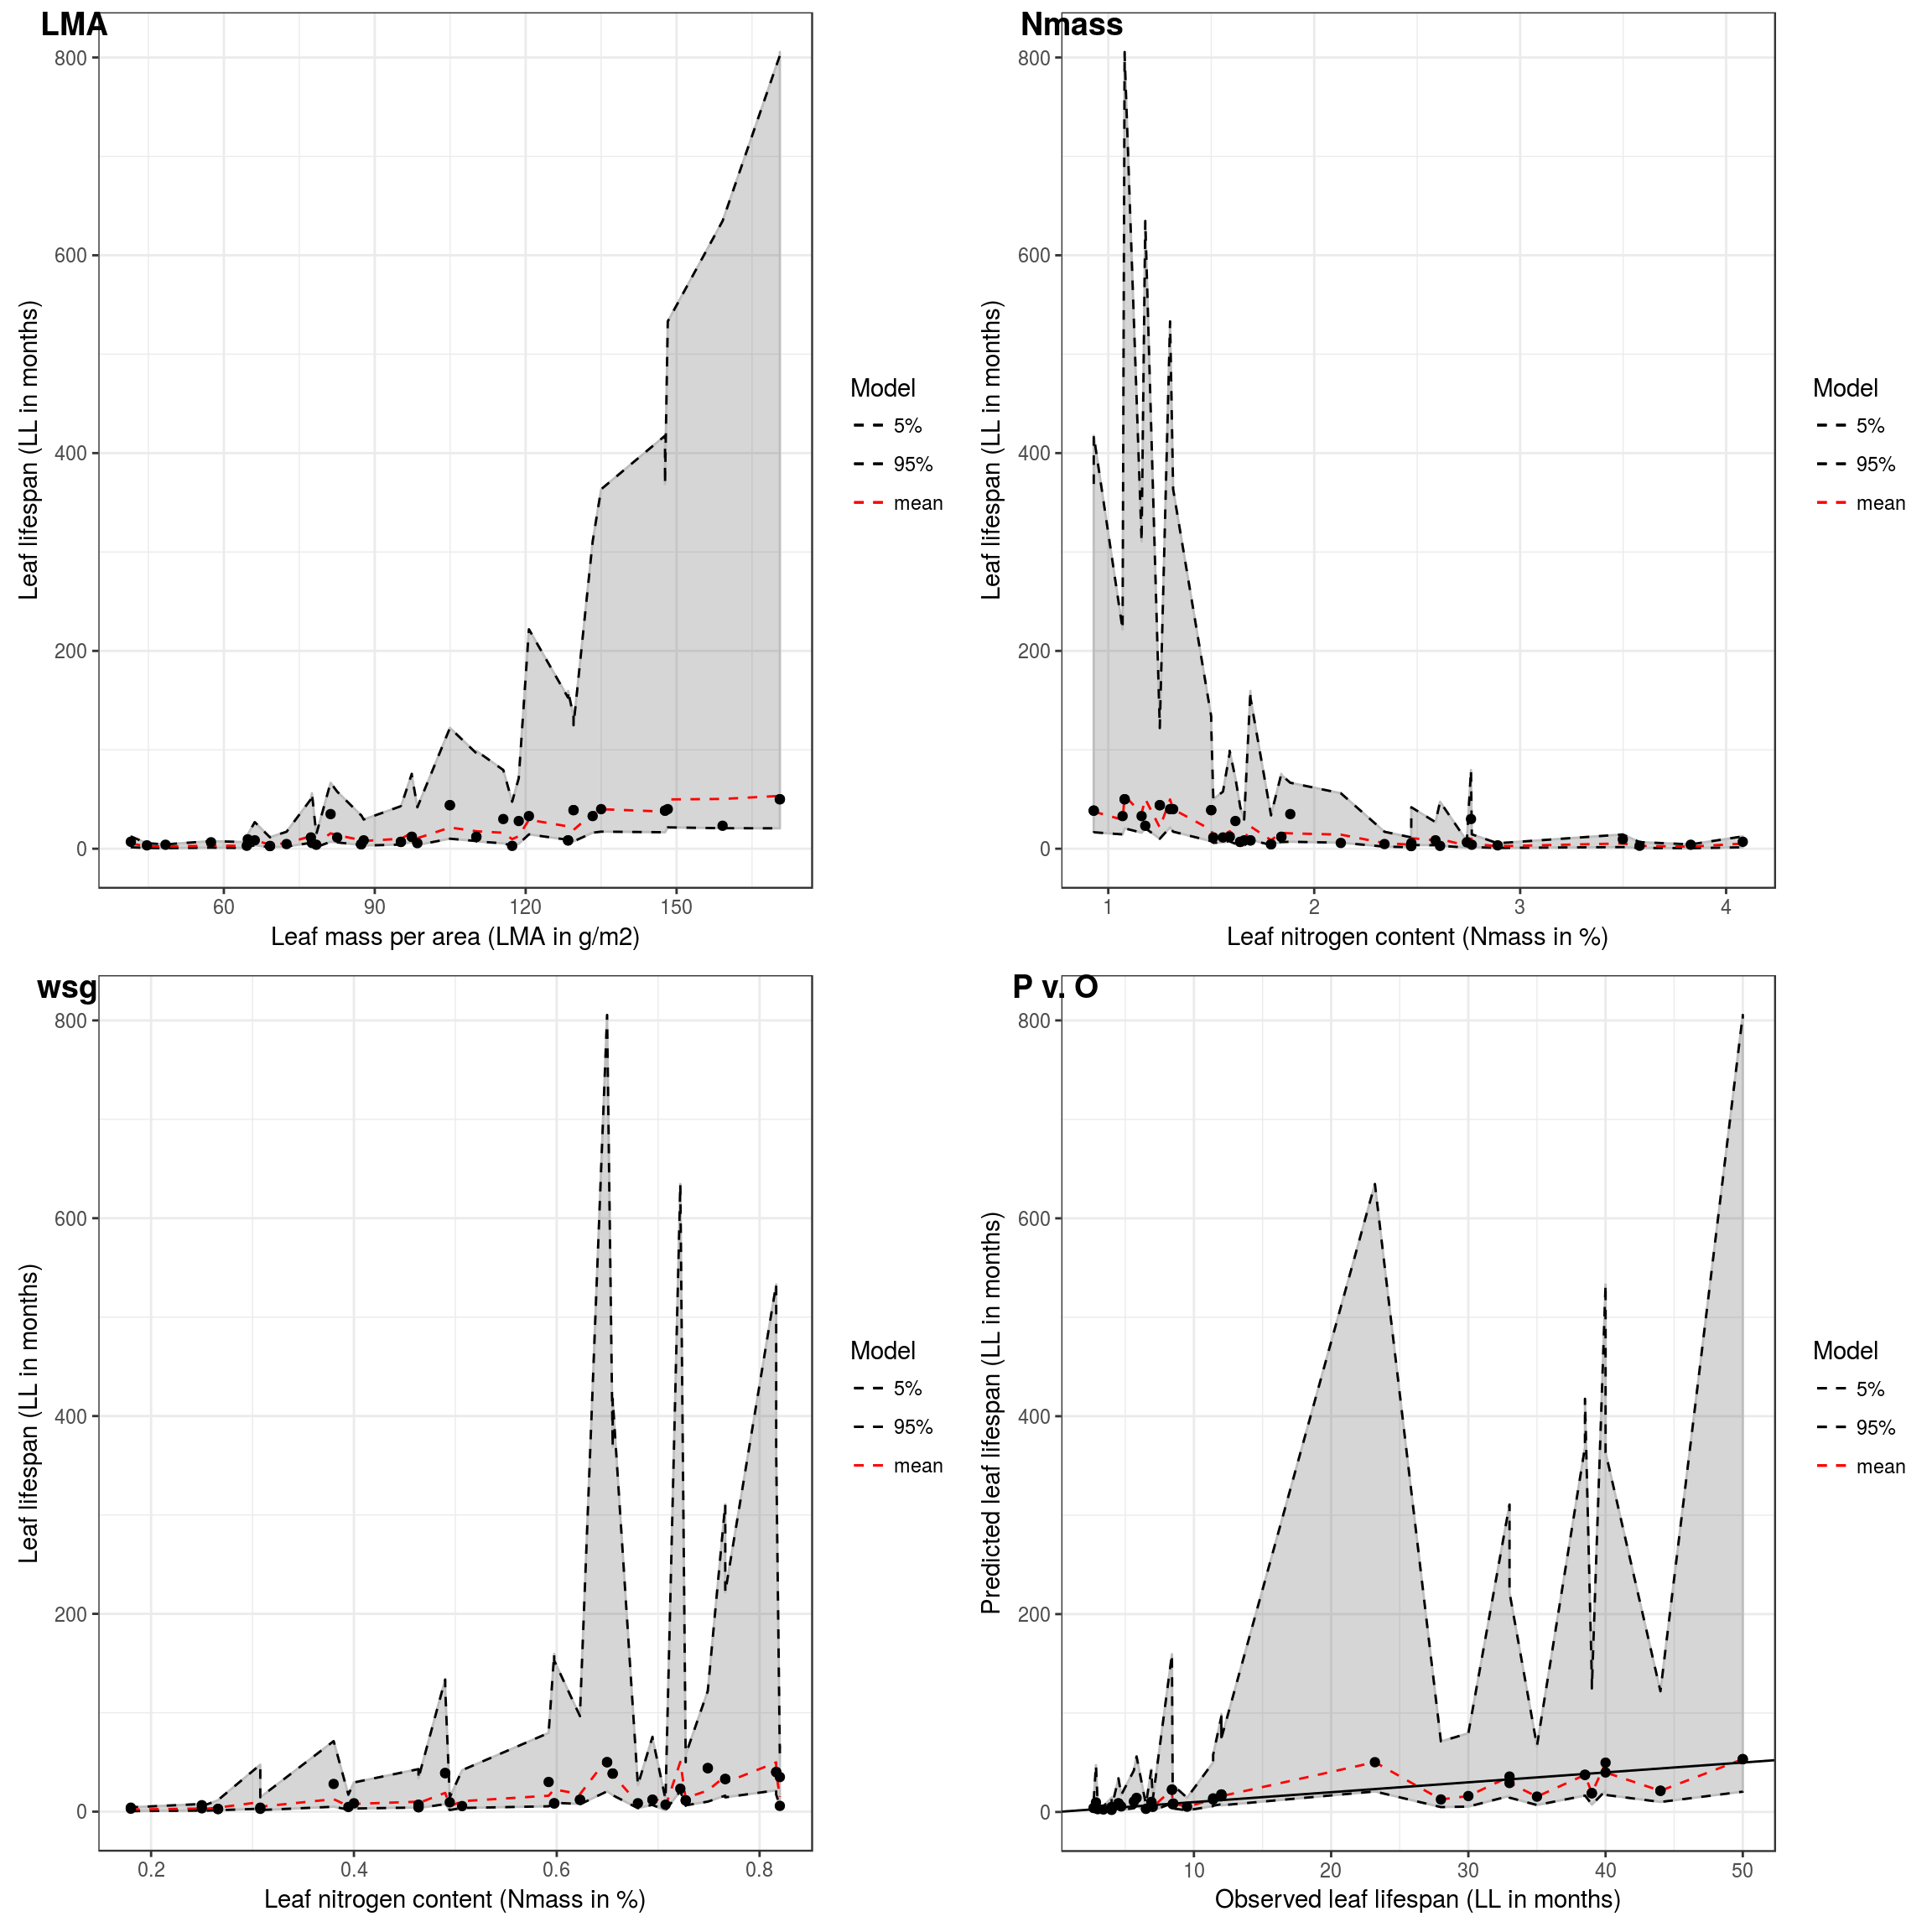
\includegraphics{master-thesis_files/figure-latex/A2LLpred-1.pdf}
\caption{\label{fig:A2LLpred}Leaflifespan predictions for the selected model
with leaf mass per area (LMA), leaf nitrogen content (Nmass), wood
specific gravity (wsg) and predicted versus observed values. Leaf
lifespan (LL) is predicted with model M10 fit. Leaf mass per area (LMA)
and leaf nitrogen content (Nmass), and wood specific gravity (wsg) are
taken in a composite dataset of GLOPNET, TRY and DRYAD datasets.Warning
LMA (resp. Nmass and wsg) is not constant and depend on the closest
point value for right (resp. center and left) graph.}
\end{figure}

Simulations are validating that this new allometry resolve the issue of
unrealistically low aboveground biomass for low LMA species due to an
early edath of individuals inside simulations. For instance with this
allometry Symphonia sp 1 (a low LMA species) is now reaching a realistic
aboveground biomass above 400 \(tonC.ha^{-1}\) and realistic diameter
and age distribution inside the final population.

\hypertarget{appendix-3-rotten-tree-model}{\section{Appendix 3: Rotten
tree model}\label{appendix-3-rotten-tree-model}}

In order to simulate sylviculture with TROLL we need to implement a new
sylviculture module inside TROLL model code. A first litterature review
was completed by an interview with Laurent Descroix of the Office
Nationale des Forêts. We discovered that rotten trees were not random
and seemed to depend both on tree species and diameter. This document
presents modelling of relation between rotten trees and their species
and diameter.

In fact we have two different questions:

\begin{itemize}
\tightlist
\item
  Predict if a tree will be probed as rotten (models \textbf{M})
\item
  Predict how much of tree volume is rotten (models \textbf{N})
\end{itemize}

First all \textbf{M} model can be written as follow:
\[Rotten_n \sim \mathcal{B}(\theta_n), ~~n \in [1,N_{=3816}] ~~ p \in [1, P_{=8}], ~~ s \in [1, S_{=43}]\]
Secondly, all \textbf{N} models depend on a latent variable being the
percentage of rotten wood \(Pt_r\). We can assume that all trees are
growing depending on species \(s\) and plot \(p\) fertility and are
supposed to have a full healthy volume \(V_h\) for a given diameter
\(dbh\). We obtain following model:

\[V_f \sim \mathcal{logN}(V_h*Pt_r, \sigma), ~~n \in [1,N_{=3268}] ~~ p \in [1, P_{=8}], ~~ s \in [1, S_{=43}]\]

We retained following models :

\begin{longtable}[]{@{}ll@{}}
\caption{\label{tab:A3models}Models summary.}\tabularnewline
\toprule
M & Model\tabularnewline
\midrule
\endfirsthead
\toprule
M & Model\tabularnewline
\midrule
\endhead
\(M_{s,p}\) &
\({P_{rotten}}_n \sim \mathcal{B}(inv_{logit}(\beta_0 + \beta_1*dbh_n + {\beta_2}_p + {\beta_3}_s))\)\tabularnewline
\(N_{s,p} + L_{s,p}\) &
\(Volume_{of~wood} \sim \mathcal{logN} (log[((\beta + \beta_p + \beta_s)*dbh^2)*(1 - Pr*((\theta + \theta_p + \theta_s) *dbh^2))], \sigma)\)\tabularnewline
\bottomrule
\end{longtable}

\subsection{Probed rotten (M)}\label{probed-rotten-m}

Based on complexity (number of parameters), convergence and likelihood
we selected model \(M_{p,s}\):

\(M_{s,p}\):
\({P_{rotten}}_n \sim \mathcal{B}(inv_{logit}(\beta_0 + \beta_1*dbh_n + {\beta_2}_p + {\beta_3}_s))\)

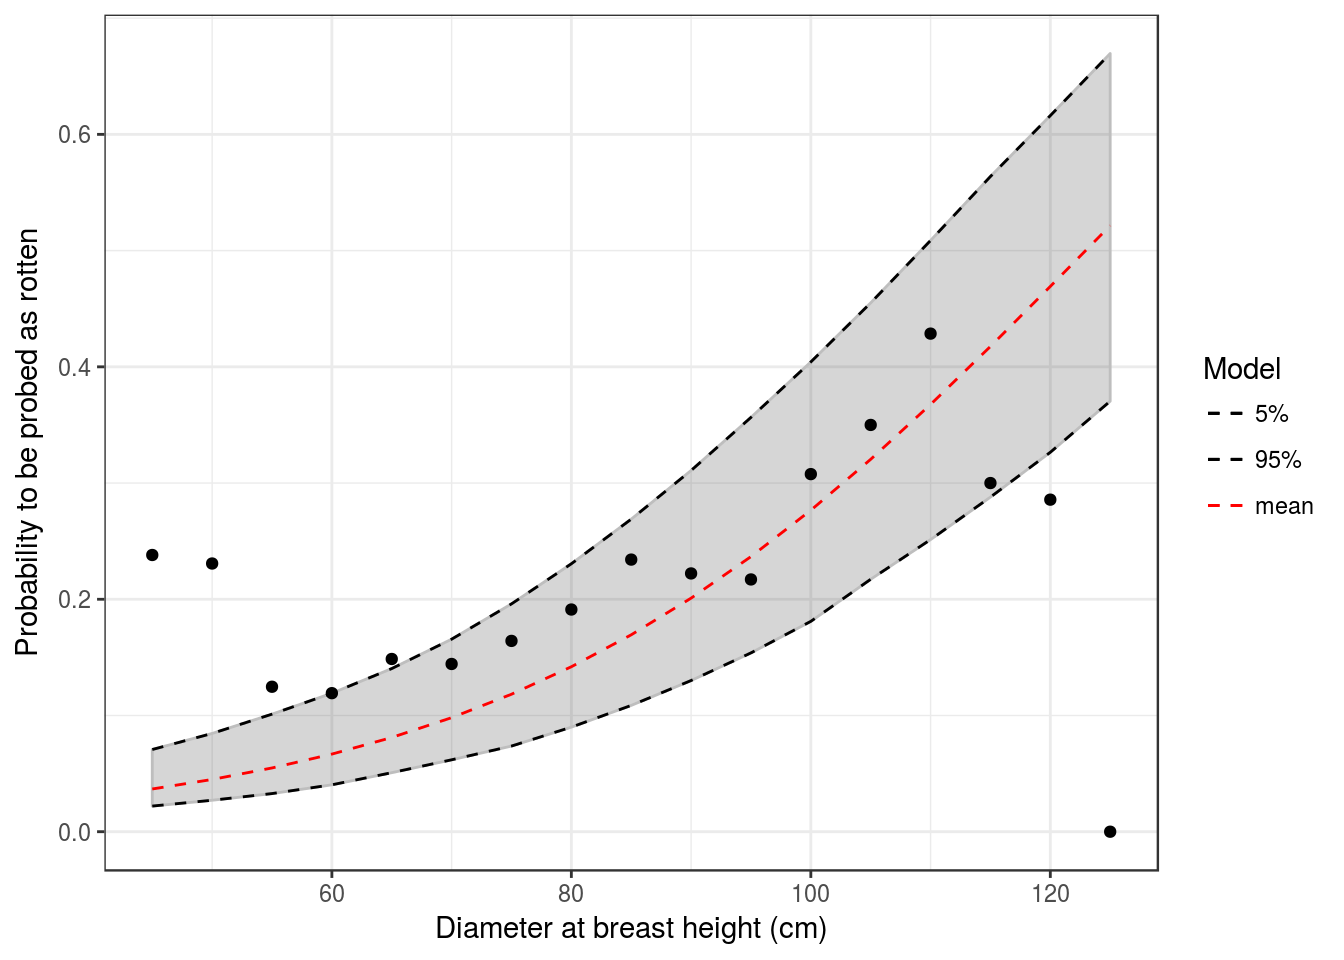
\includegraphics{master-thesis_files/figure-latex/A3Mpred-1.pdf}

\begin{longtable}[]{@{}lrrrrrrrrrrrrrrrrr@{}}
\caption{\label{tab:A3Mtab}Models prediction. Probability to be probed as
rotten (P in \%) for a given dbh (cm).}\tabularnewline
\toprule
& 45 & 50 & 55 & 60 & 65 & 70 & 75 & 80 & 85 & 90 & 95 & 100 & 105 & 110
& 115 & 120 & 125\tabularnewline
\midrule
\endfirsthead
\toprule
& 45 & 50 & 55 & 60 & 65 & 70 & 75 & 80 & 85 & 90 & 95 & 100 & 105 & 110
& 115 & 120 & 125\tabularnewline
\midrule
\endhead
P & 4 & 4 & 5 & 7 & 8 & 10 & 12 & 14 & 17 & 20 & 24 & 28 & 32 & 37 & 42
& 47 & 52\tabularnewline
\bottomrule
\end{longtable}

\subsection{Rotten volume (N)}\label{rotten-volume-n}

Based on complexity (number of parameters), convergence and likelihood
we selected model \(N_{p,s}\) associated to hyperparameter \(\rho\) with
model \(L_{p,s}\):

\(N_{s,p} + L_{s,p}\):
\(Volume_{of~wood} \sim \mathcal{logN} (log[((\beta + \beta_p + \beta_s)*dbh^2)*(1 - Pr*((\theta + \theta_p + \theta_s) *dbh^2))], \sigma)\)

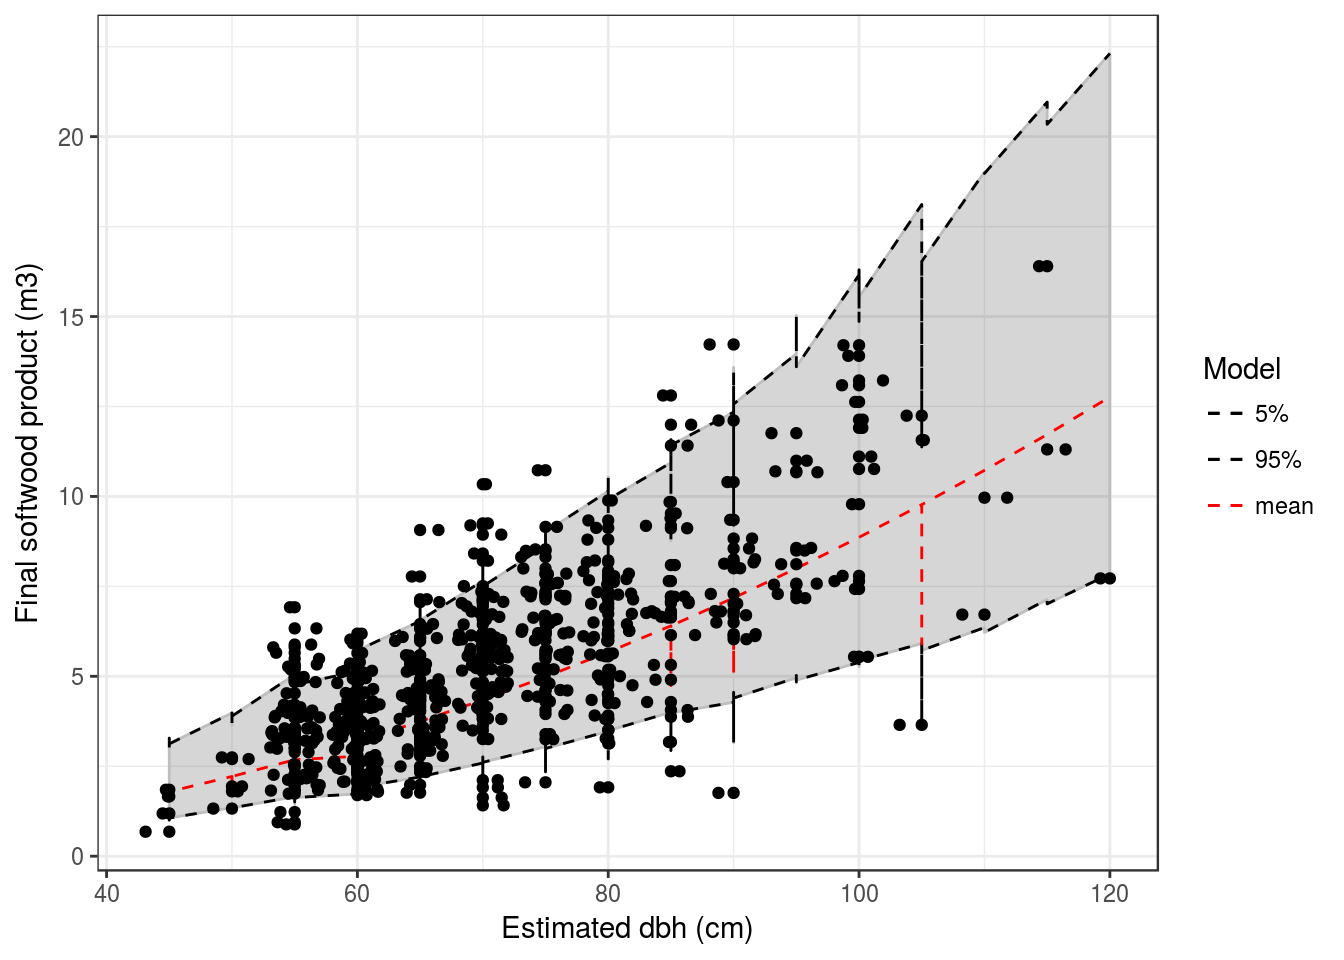
\includegraphics{master-thesis_files/figure-latex/A3Npred-1.pdf}

\begin{longtable}[]{@{}lrrrrrrrrrrrrrrrrr@{}}
\caption{\label{tab:A3Ntab}Models prediction. Final volume of wood (\(V_f\)
in \(m^3\)) and percent of rotten wood (\(V_p\) in \%) for a given dbh
(cm) if the tree was probed rotten.}\tabularnewline
\toprule
& 45 & 50 & 55 & 60 & 65 & 70 & 75 & 80 & 85 & 90 & 95 & 100 & 105 & 110
& 115 & 120 & 125\tabularnewline
\midrule
\endfirsthead
\toprule
& 45 & 50 & 55 & 60 & 65 & 70 & 75 & 80 & 85 & 90 & 95 & 100 & 105 & 110
& 115 & 120 & 125\tabularnewline
\midrule
\endhead
Vf & 1.66 & 2.02 & 2.39 & 2.78 & 3.18 & 3.58 & 3.98 & 4.37 & 4.74 & 5.09
& 5.41 & 5.68 & 5.9 & 6.06 & 6.15 & 6.16 & 6.08\tabularnewline
Vp & 7.00 & 9.00 & 11.00 & 13.00 & 15.00 & 18.00 & 20.00 & 23.00 & 26.00
& 29.00 & 32.00 & 36.00 & 40.0 & 43.00 & 47.00 & 52.00 &
56.00\tabularnewline
\bottomrule
\end{longtable}

\section{Appendix 4: Sensitivity
analysis}\label{appendix-4-sensitivity-analysis}

To study resistance and resilience of ecosystem face to disturbance,
highlighting the role of biodiversity, we decided to use TROLL model
simulations \citep{Chave1999}. In order to get a finer study of
simulations response, we need to assess first sensitivity of the TROLL
model to different parameters. More particularly we need to assess the
importance of functional traits to further better control functional
diversities in simulations. We also need to assess sensitivity of the
model to see rain constant because we assume it is one of the main
factor of tree recruitments after disturbance in the model.

\subsection{Material and methods}\label{material-and-methods-2}

To assess the sensitivity of TROLL model to species functionnal traits,
we performed a sensitivity analysis by fixing species trait values to
their mean. Each trait was tested independently. We reduce to a common
mean traits with a correlation \(r \geq 0.8\) (see figure
\ref{fig:A4corr}).

\begin{figure}[htbp]
\centering
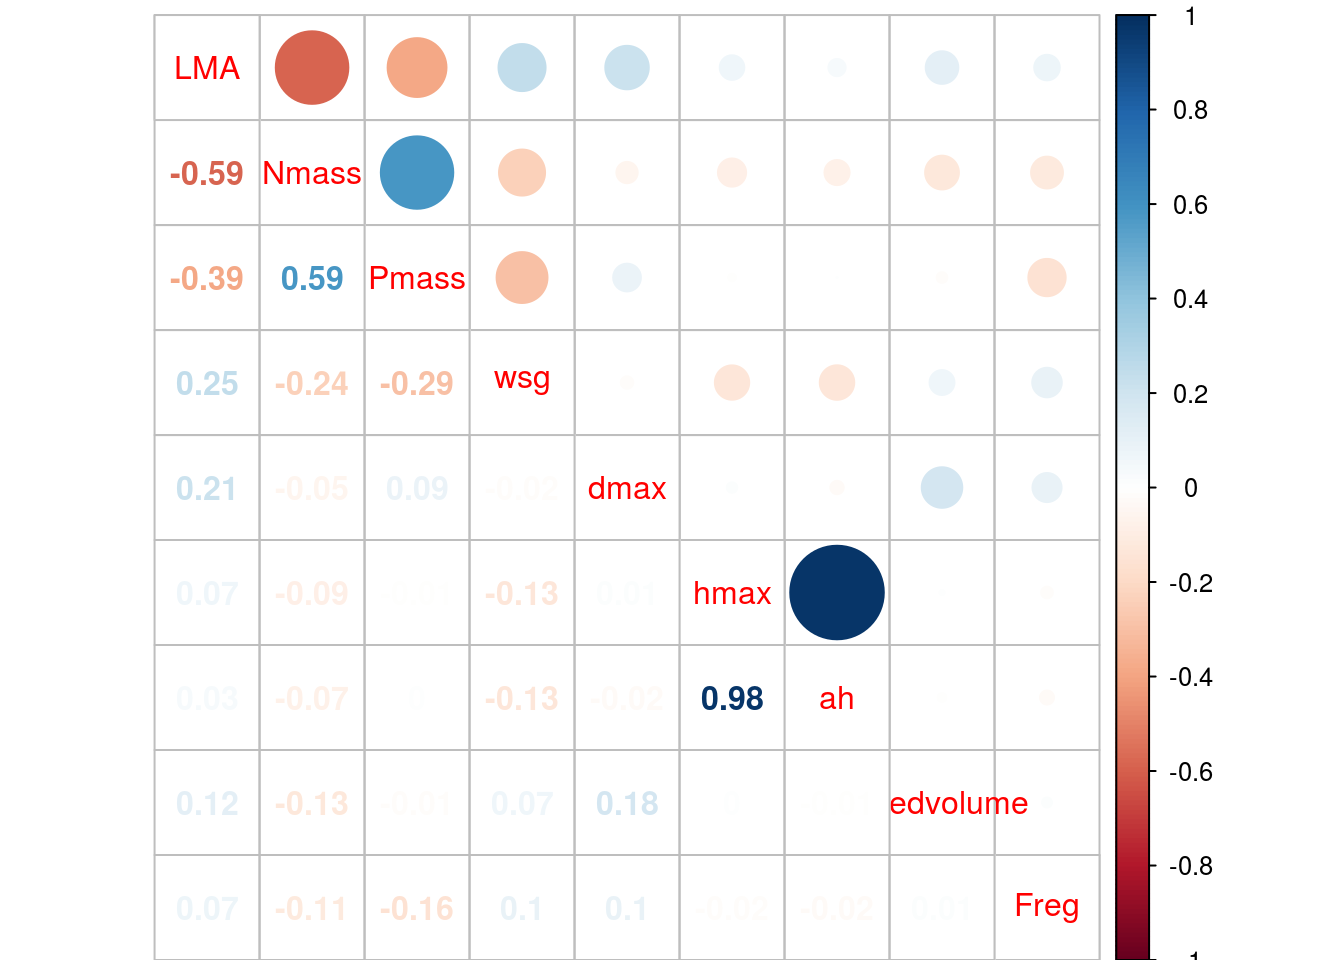
\includegraphics{master-thesis_files/figure-latex/A4corr-1.pdf}
\caption{\label{fig:A4corr}Correlation of functional traits within TROLL
model species Blue represents negative coorelations whereas red
represents positive correlations. Values and colour intensity represents
correlation values.}
\end{figure}

To assess the sensitivity of TROLL model to seed rain, we performed a
sensitivity analysis by fixing simulations seed rain constant to 2, 20,
200 and 2000 seeds per hectare.

Simulations were conducted on Intel Xeon(R) with 32 CPUs of 2.00GHz and
188.9 GB of memory. We assumed maturity of the forest after 500 years of
regeneration \citep{Li} and computed simulation 100 years after a
disturbance event of 40\% intensity. Due to computer limitations we did
not run replicate (besides it should be necessary to reduce simulation
stochasticity). To assess ecosystem outputs sensitivity to studied
parameters, we compared it to 100 replicates of control simulations with
all parameters set to default values. Ecosystem outputs outside of the
range of the control replicates values are significantly influenced by
the studied parameter.

\subsection{Results}\label{results-2}

\subsubsection{Control}\label{control}

Both disturbed ecosystem structure and functional composition
corresponded to ecosystem structure and functional composition before
disturbance (figure \ref{fig:A4controlStr}). Consequently, we assumed
that disturbance did not affect much ecosystem structure and function.
Secondly range of values inside control replicates is low (figure
\ref{fig:A4controlVar}).

\begin{figure}[htbp]
\centering
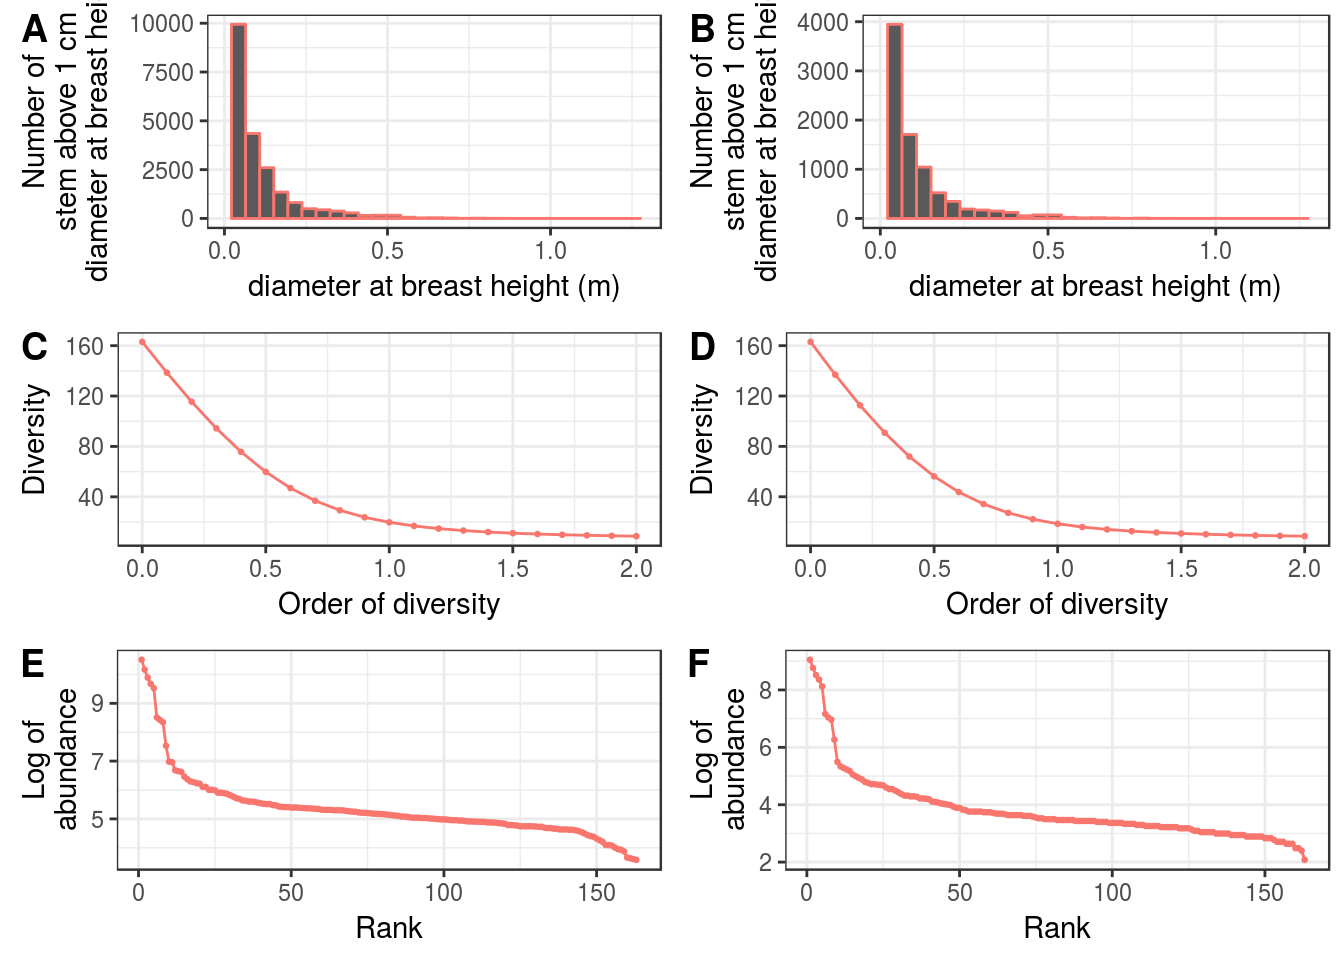
\includegraphics{master-thesis_files/figure-latex/A4controlStr-1.pdf}
\caption{\label{fig:A4controlStr}Ecosystem structure before disturbance and
disturbed. Ecosystem structure before disturbance (left) and disturbed
(right) with diameter structure (A, B), diversity at different orders
(C, D) and rank-abundance diagrams (E, F).}
\end{figure}

\begin{figure}[htbp]
\centering
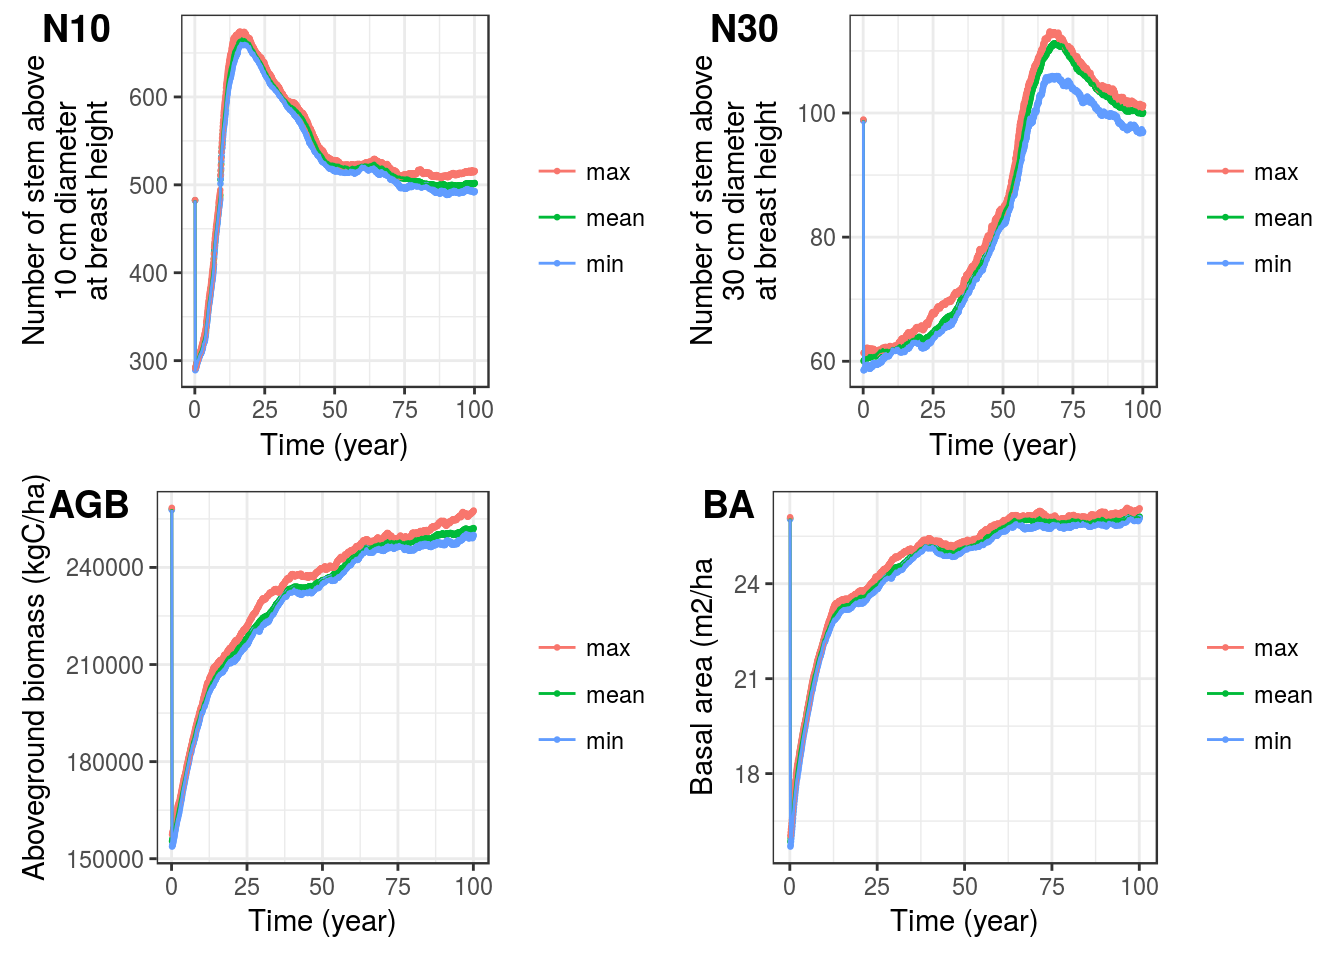
\includegraphics{master-thesis_files/figure-latex/A4controlVar-1.pdf}
\caption{\label{fig:A4controlVar}Control replicates variation. Maximum, mean
and minimum number of trees with dbh above 10 cm (N10) and 30 cm (N30),
above ground biomass (AGB) and basal area (BA) over simulation time.}
\end{figure}

\subsubsection{Functional traits}\label{functional-traits}

Most of functional traits had a significant long term influence on
ecosystem outputs (figure \ref{fig:A4ftVar}). Only \textbf{seed volume}
was always in the range of variation of control replicates. On the other
hand, few functional traits influenced final ecosystem structure (figure
\ref{fig:A4ftStr}). Only specific maximum diameter \textbf{dmax} add
higher diversity for greater orders implying better eveness in species
distributions. Regarding functional composition, traits fixed to mean
did not change other functional traits density distribution.

\textbf{ah-hmax} traits fixed to mean increased number of stems above 10
and above 30 cm dbh and basal area after disturbance (but not in long
term) and did not affect aboveground biomass. Similarly, wood specific
gravity \textbf{wsg} trait fixed to mean had exactly the same effect on
number of stems above 10 and above 30 cm dbh and basal area after
disturbance than \textbf{ah-hmax} but with a time lag ; and \textbf{wsg}
also increased aboveground biomass. \textbf{dmax} trait fixed to mean
slightly decreased number of stems above 10 and above 30 cm dbh over
time while it increased basal area, aboveground biomass, and species
eveness. Finally, leaf mass per area \textbf{LMA} trait fixed to mean
only decreased number of stem above 10 cm dbh after ecosystem resilience
to disturbance (approximately 50 years) but did not affect other
ecosystem outputs.

\begin{figure}[htbp]
\centering
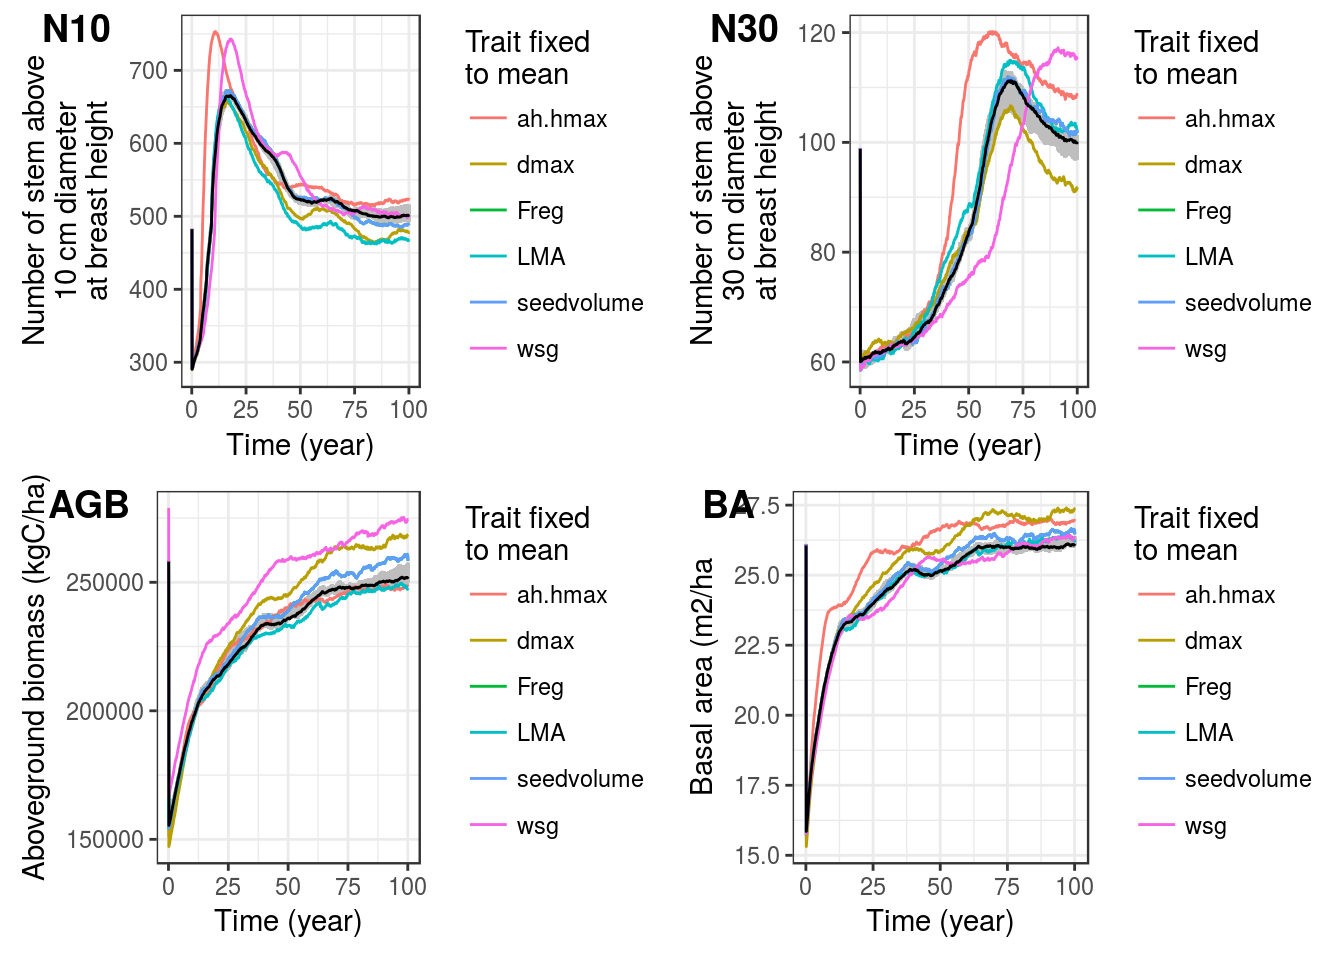
\includegraphics{master-thesis_files/figure-latex/A4ftVar-1.pdf}
\caption{\label{fig:A4ftVar}Functional traits effect on simulation ecosystem
variations over time. Number of trees with dbh above 10 cm (N10) and 30
cm (N30), above ground biomass (AGB) and basal area (BA). Grey area
represents the interval of control replicates whereas black line
represents the mean of control replicates.}
\end{figure}

\begin{figure}[htbp]
\centering
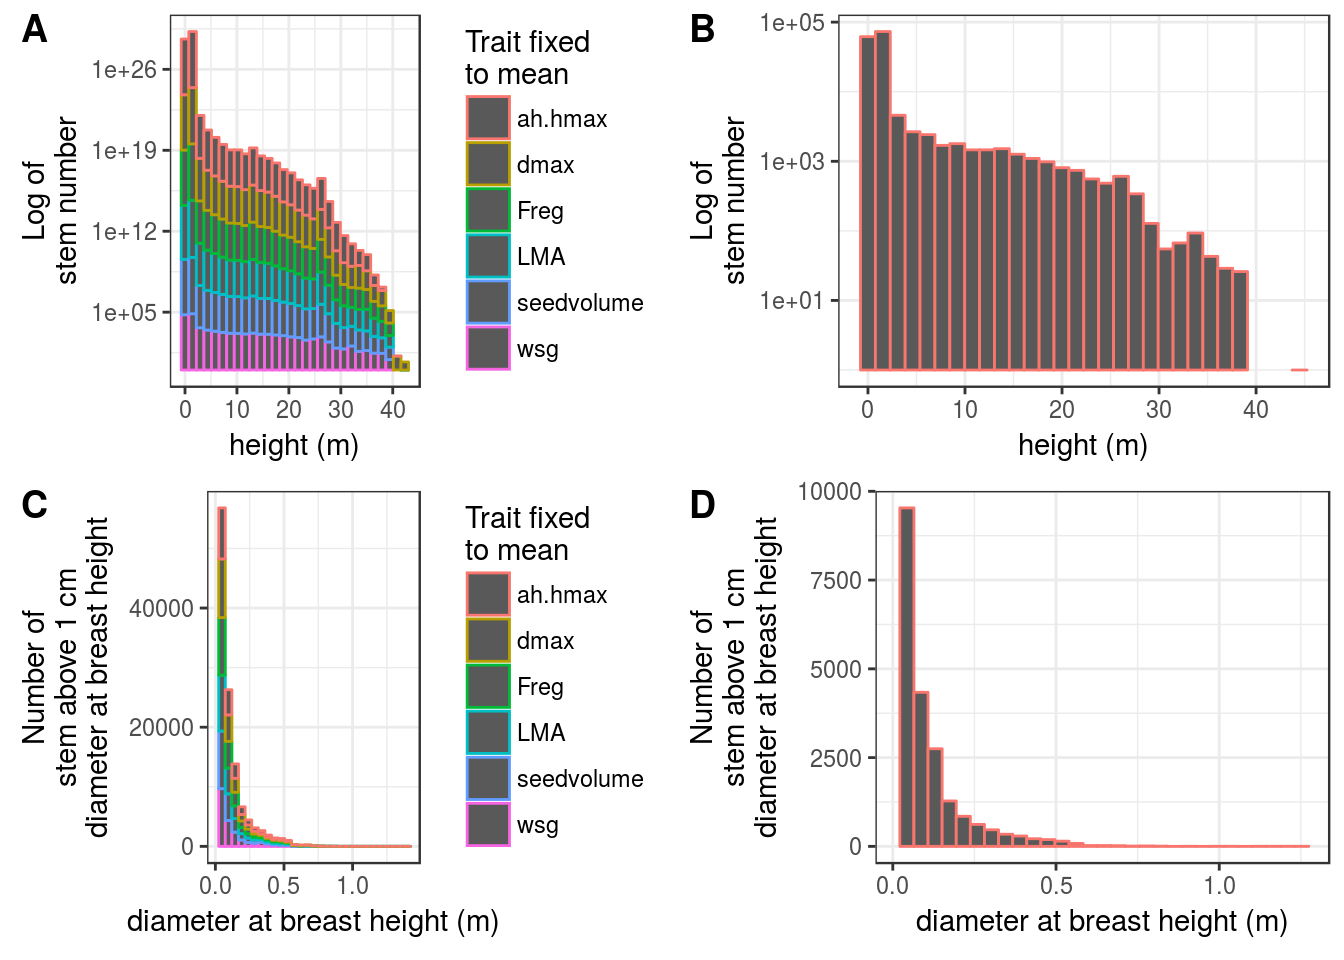
\includegraphics{master-thesis_files/figure-latex/A4ftStr-1.pdf}
\caption{\label{fig:A4ftStr}Functional traits effect on simulation ecosystem
final structure. Tree final height histogram for traits (A) and control
(B), tree final diameter histogram for traits (C) and control (D),
ecosystem final diversity plot at different orders (E), and ecosystem
final rank-abundance diagram (F).}
\end{figure}

\subsubsection{Seed rain}\label{seed-rain}

Seedrain constant affected ecosystem outputs only when set lower than
default value (figure \ref{fig:A4srVar} \& \ref{fig:A4srStr}). Moreover,
seedrain did not seem to affect aboveground biomass (figure
\ref{fig:A4srVar}) and final ecosystem height and diameter structure
(figure \ref{fig:A4srStr}). Seedrain constant fixed to 2 or 20 seed per
hectare seemed to have a similar effect. Lower seedrain implied faster
decrease of stem above 10 cm dbh and higher number of stem above 30 cm
dbh after ecosystem resilience to disturbance (approximately 50 years).
Lower seedrain than default decreased basal area over time. In addition,
lower seedrain than default decreased equitability by increasing
abundance of abundant species and decreasing abundance of less abundant
species. Seedrain constant even decreased the total number of species
when fixed to 2 seed per hectare. Finally, seedrain constant slightly
affected functional composition with higher pike on ecosystem most
representatives functional trait values. In a nutshell, the lower is the
seedrain constant the most the functional density distribution is
aggregated around few functional trait values.

\begin{figure}[htbp]
\centering
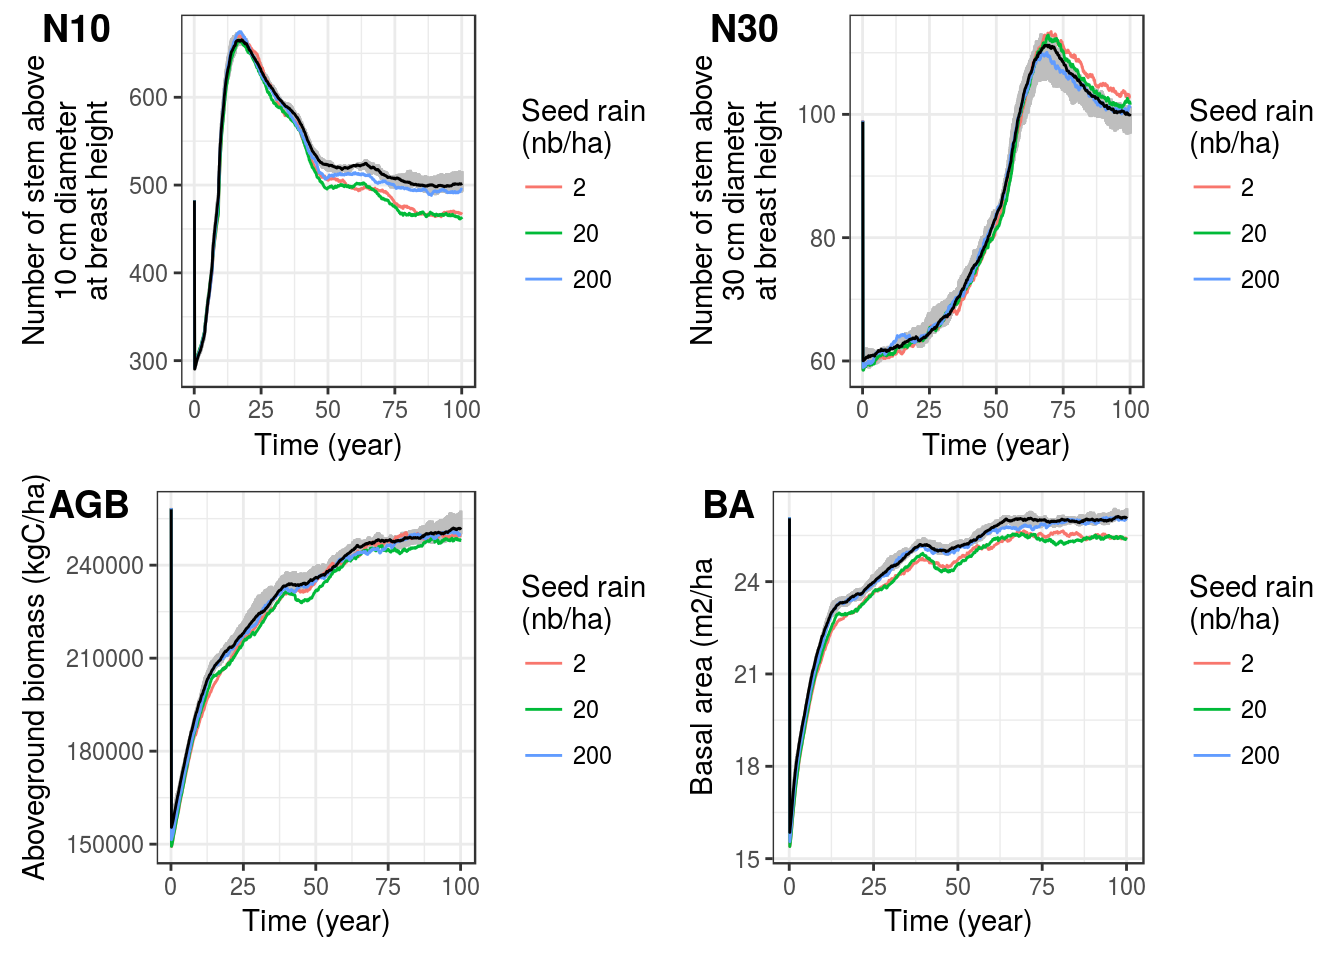
\includegraphics{master-thesis_files/figure-latex/A4srVar-1.pdf}
\caption{\label{fig:A4srVar}Seed rain effect on simulation ecosystem
variations over time. Number of trees with dbh above 10 cm (N10) and 30
cm (N30), above ground biomass (AGB) and basal area (BA). Grey area
represents the interval of control replicates whereas black line
represents the mean of control replicates.}
\end{figure}

\begin{figure}[htbp]
\centering
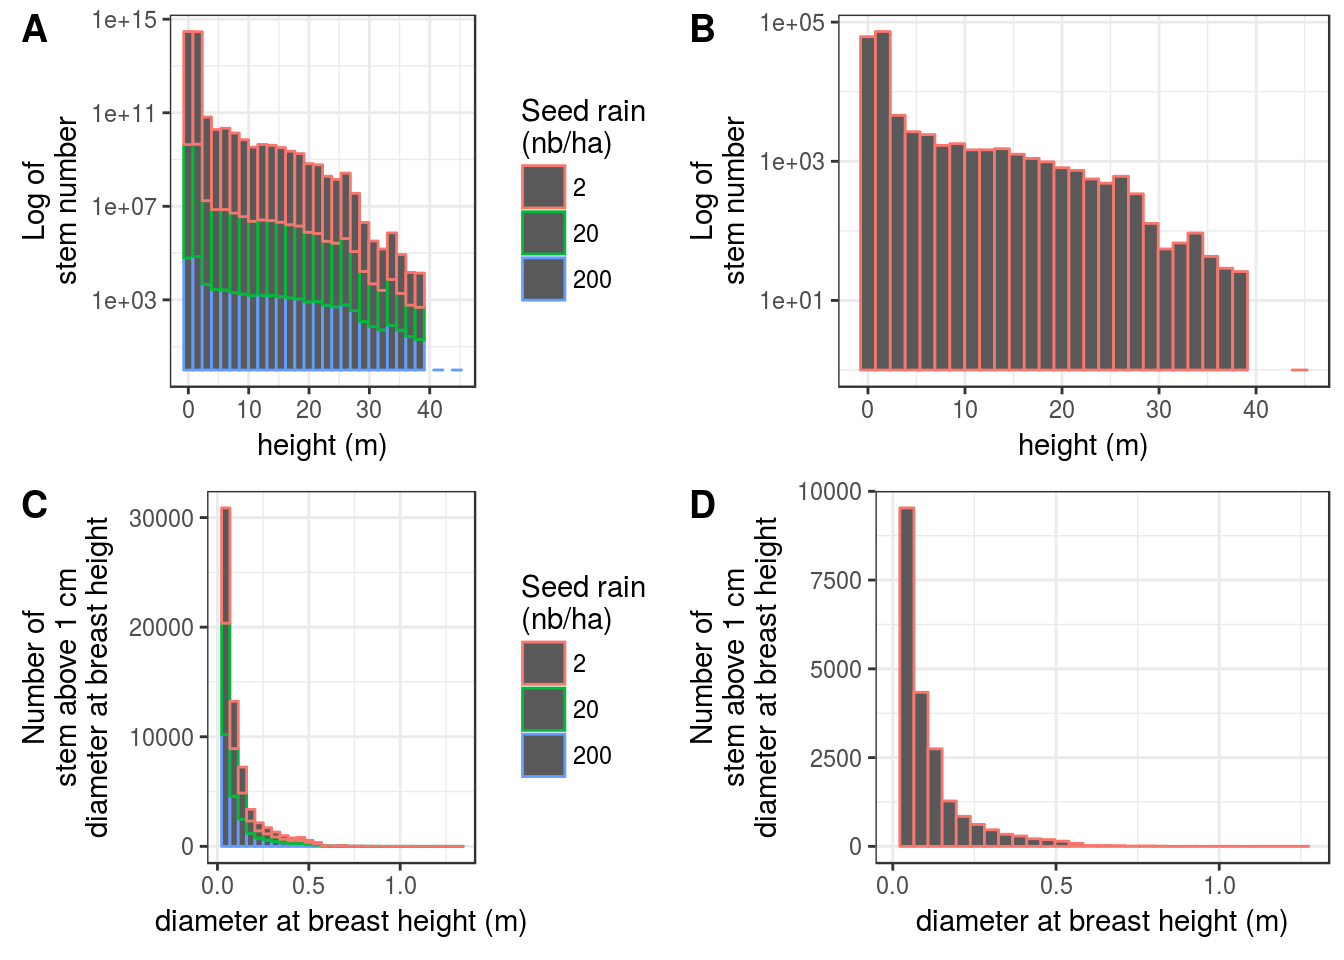
\includegraphics{master-thesis_files/figure-latex/A4srStr-1.pdf}
\caption{\label{fig:A4srStr}Seed rain effect on simulation ecosystem final
structure. Tree final height histogram for traits (A) and control (B),
tree final diameter histogram for traits (C) and control (D).}
\end{figure}

\subsection{Discussion}\label{discussion-1}

\subsubsection{Disturbance simulation}\label{disturbance-simulation}

Ecosystem structure, species organisation and functional composition
stayed the same before and after disturbance. We can thus validate
disturbance module in its actual state. Morevoer we can now consider
that the composition we will initialise at the beginning of simulations
will stay the same after disturbance. Finally control replicates has
shown few stochasticity, it advocates for few or no replicates in
further analysis.

\subsubsection{Functional traits
selection}\label{functional-traits-selection}

\textbf{ah-hmax} fixed to mean implied no high or low trees. Less high
trees left space for more trees increasing number of stems in the
ecosystem thus increasing basal area. Wood specific gravity \textbf{wsg}
fixed to mean mainly increased wood density of light wood species.
Globally higher wood density increased lifespan of individuals
responsible for the time lag and the higher number of stems increasing
basal area. \textbf{wsg} fiwed to mean also increased carbon capture by
individuals, thus increasing aboveground biomass. Specific maximum
diameter \textbf{dmax} fixed to mean decreased death rates. Decreased
death rate diminished number of stems, expecially big ones thus
increasing global basal area and abiveground biomass. \textbf{dmax}
fixed to mean by keeping more small diameter stems also increased random
selection of species increasing eveness in species distribution.
Considering the high correlation between \textbf{ah} and \textbf{hmax}
we could also keep only \textbf{hmax} (because of its more
straightforward ecological meaning).

\subsubsection{Seed rain constant
influence}\label{seed-rain-constant-influence}

Seedrain constant did not directly affect ecosystem global outputs over
simulation post-disturbance time but have a major effect on species and
functional composition and diversity. Reducing seedrain constant
resulted in an ecosystem selecting few species increasing their
abundance and functional dominance of their traits. Thus reduced
seedrain constant greatly diminsihed eveness untill a decrease of total
number of species for its lowest value.

\hypertarget{appendix-5-disturbance-simulations}{\section{Appendix 5:
Disturbance simulations}\label{appendix-5-disturbance-simulations}}

\subsection{Ecosystem functions}\label{ecosystem-functions-2}

Appendix 4 presents ecosystem resilience after 600 years with taxonomic
and functional diversity for different levels of disturbance. It
encompass all functionnal diversity components \citep[FRIC, FEve, FDiv,
and FDis,][]{villeger_new_2008}. And it presents results for both forest
dynamic (Figure \ref{fig:A4IeqStructureAll}) and forest production
(Figure \ref{fig:A4IeqProductionAll}).

\begin{verbatim}
## 
## Attaching package: 'dplyr'
\end{verbatim}

\begin{verbatim}
## The following objects are masked from 'package:stats':
## 
##     filter, lag
\end{verbatim}

\begin{verbatim}
## The following objects are masked from 'package:base':
## 
##     intersect, setdiff, setequal, union
\end{verbatim}

\begin{figure}[htbp]
\centering
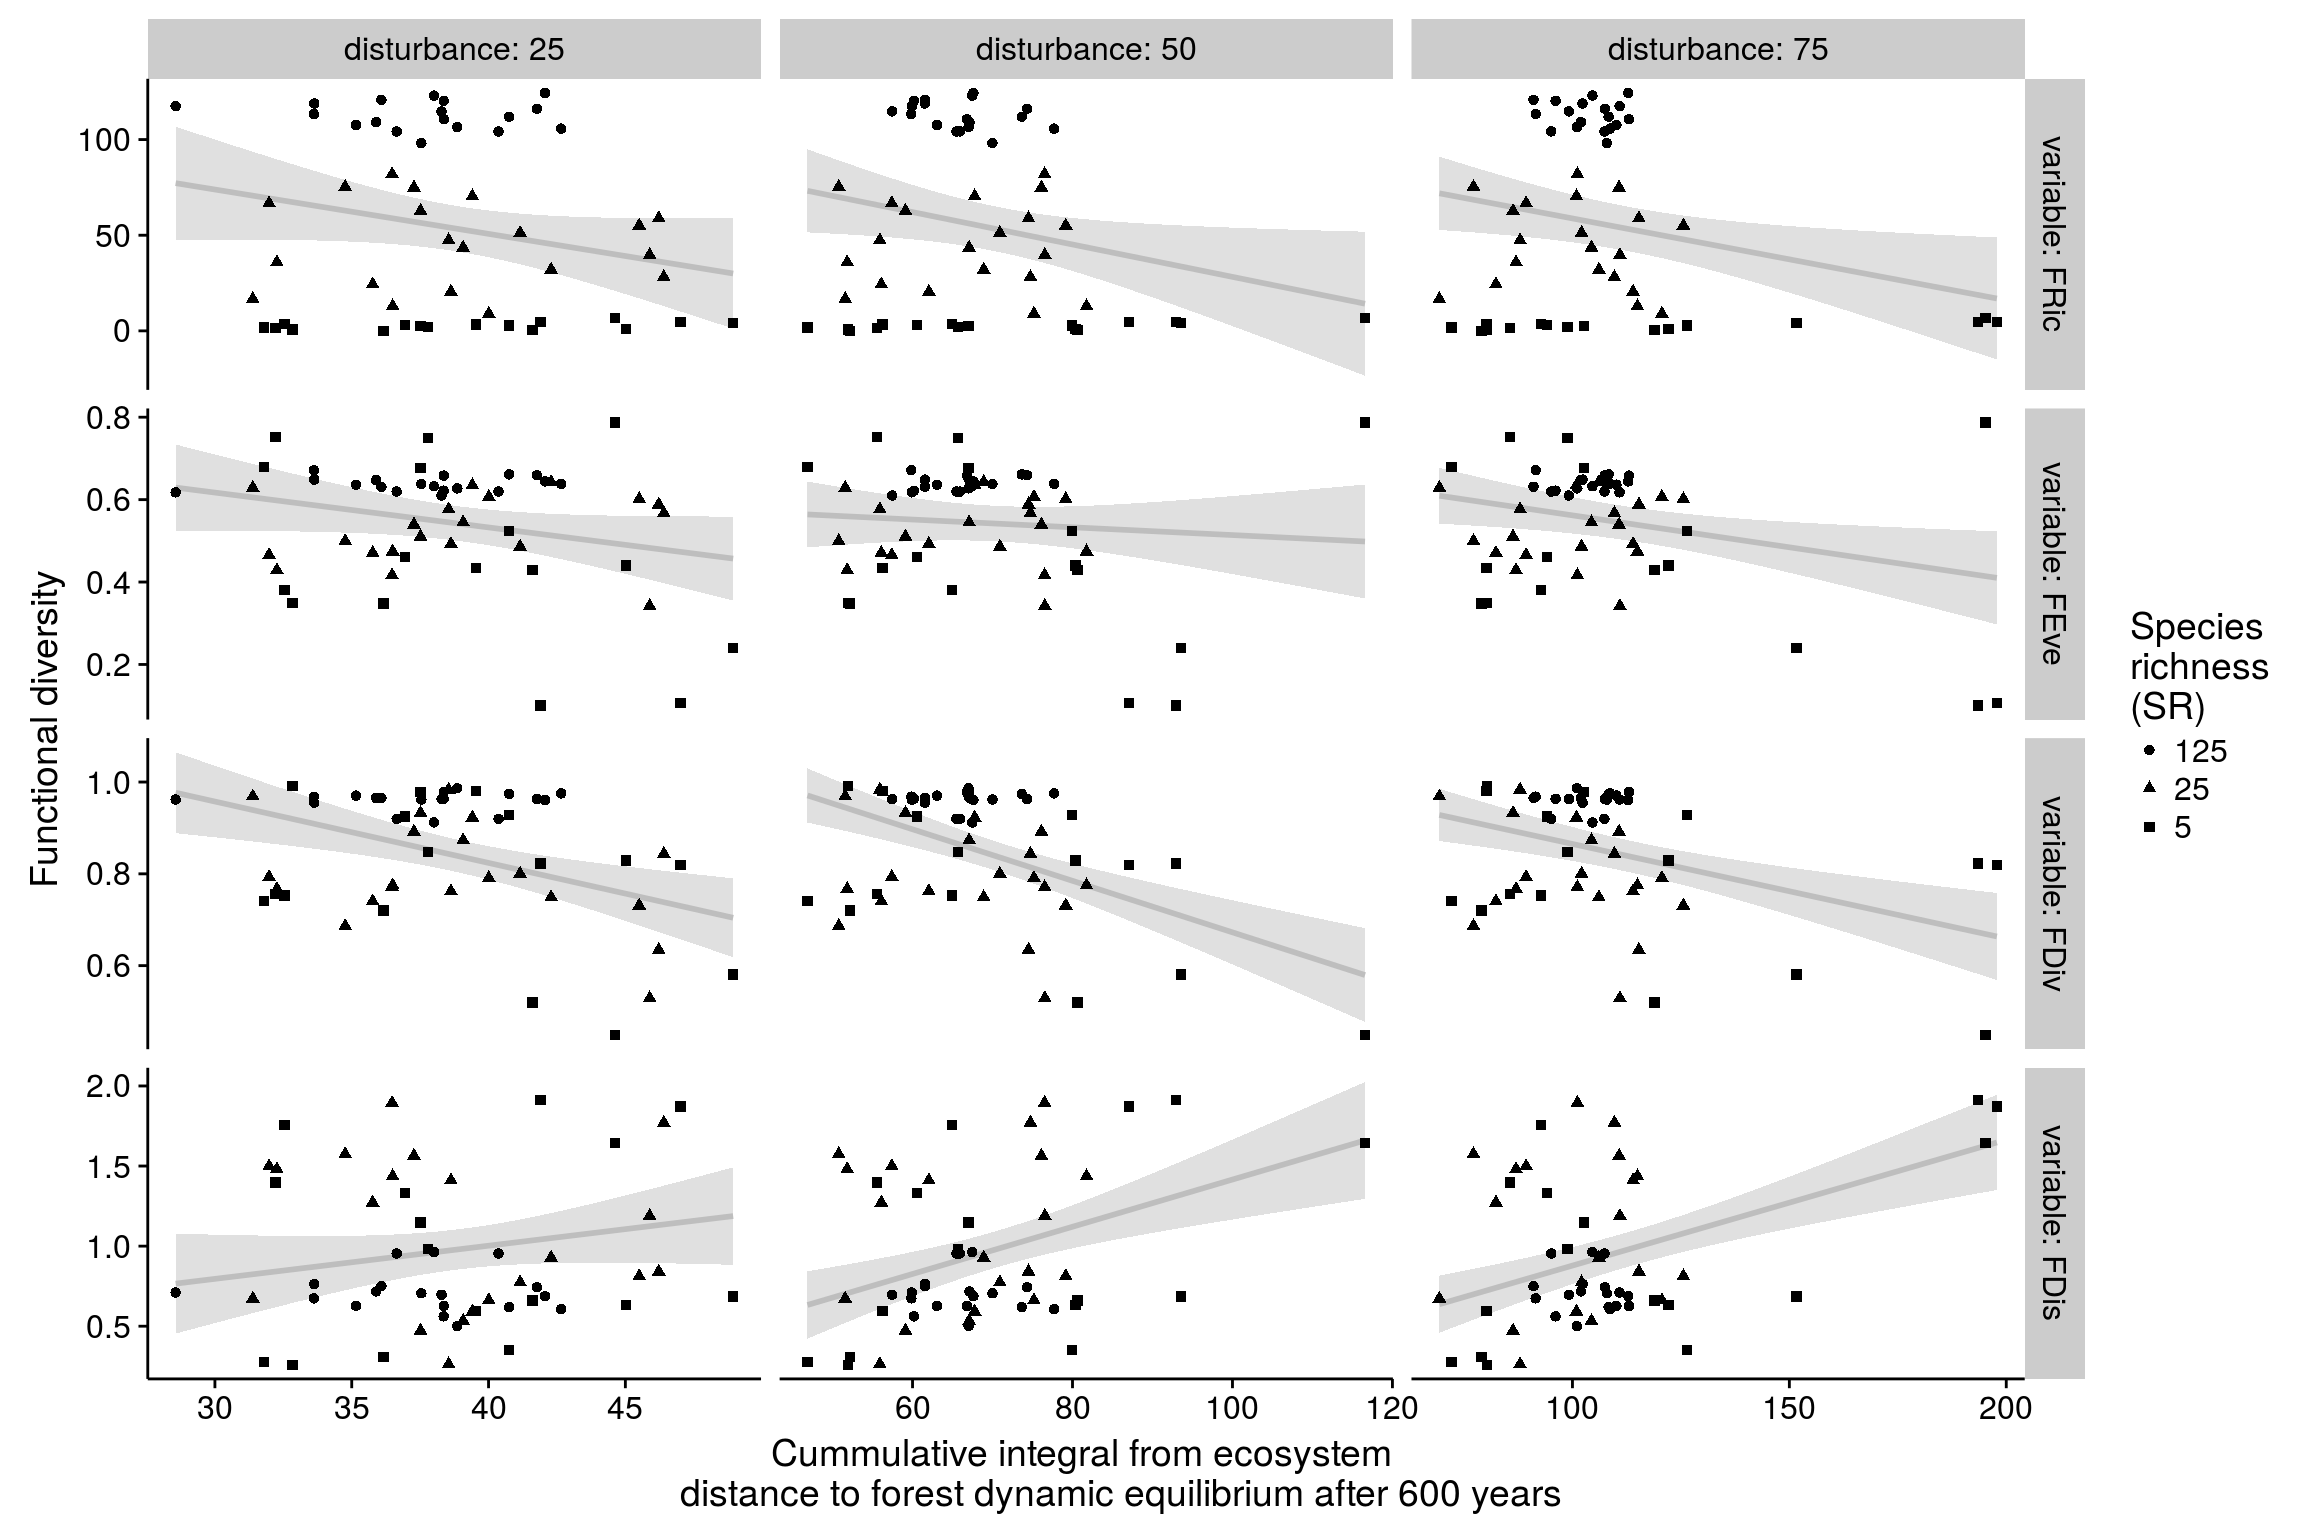
\includegraphics{master-thesis_files/figure-latex/A5IeqStructureAll-1.pdf}
\caption{\label{fig:A5IeqStructureAll}Ecosystem resilience after 600 years
with taxonomic and functional diversity for different levels of
disturbance. Cummulative integral from ecosystem distance to forest
dynamic equilibrium after 600 years was represented against functional
diversity \citep[FRIC, FEve, FDiv, and FDis,][]{villeger_new_2008} for
different level of disturbance (25, 50 and 75\% of total basal area);
dot shapes represents the species richness.}
\end{figure}

\begin{figure}[htbp]
\centering
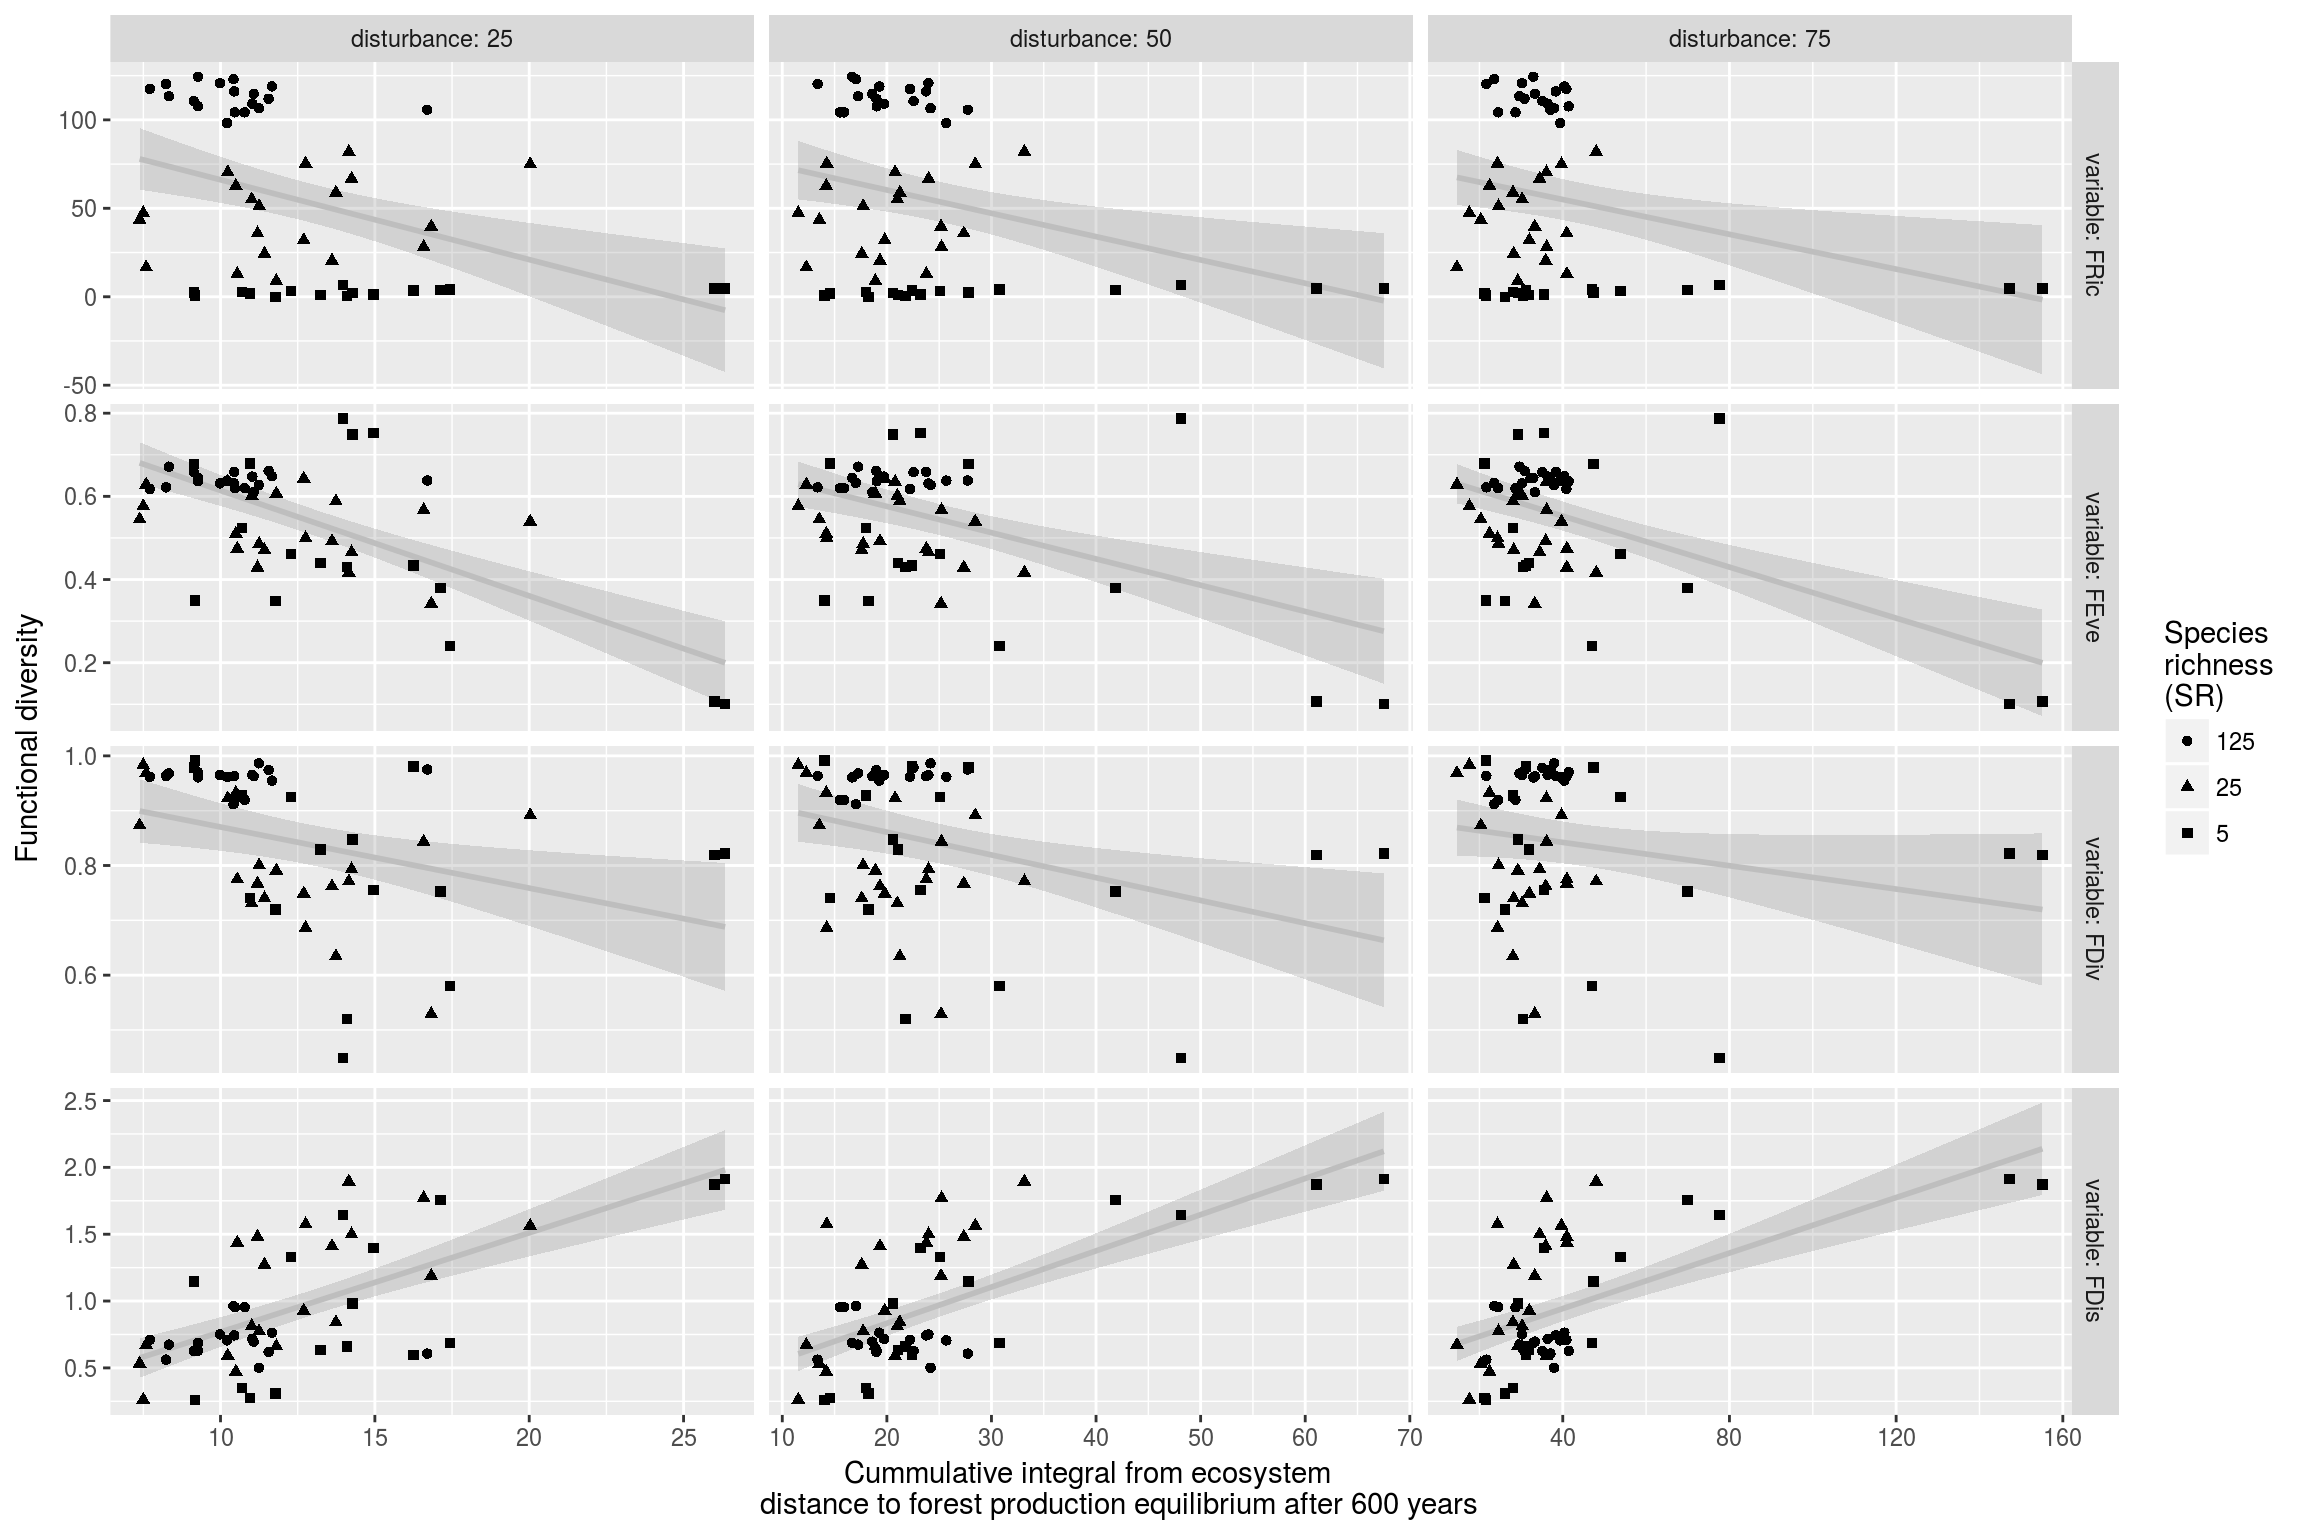
\includegraphics{master-thesis_files/figure-latex/A5IeqProductionAll-1.pdf}
\caption{\label{fig:A5IeqProductionAll}Ecosystem resilience after 600 years
with taxonomic and functional diversity for different levels of
disturbance. Cummulative integral from ecosystem distance to forest
production equilibrium after 600 years was represented against
functional diversity \citep[FRIC, FEve, FDiv, and
FDis,][]{villeger_new_2008} for different level of disturbance (25, 50
and 75\% of total basal area); dot shapes represents the species
richness.}
\end{figure}

\subsection{Biodiversity effect}\label{biodiversity-effect-2}

Figure \ref{fig:A4allBE} presents the resilience of complementarity and
selection effects for different ecosystem metrics (AGB, BA, N, GPP and
NPP).

\begin{figure}[htbp]
\centering
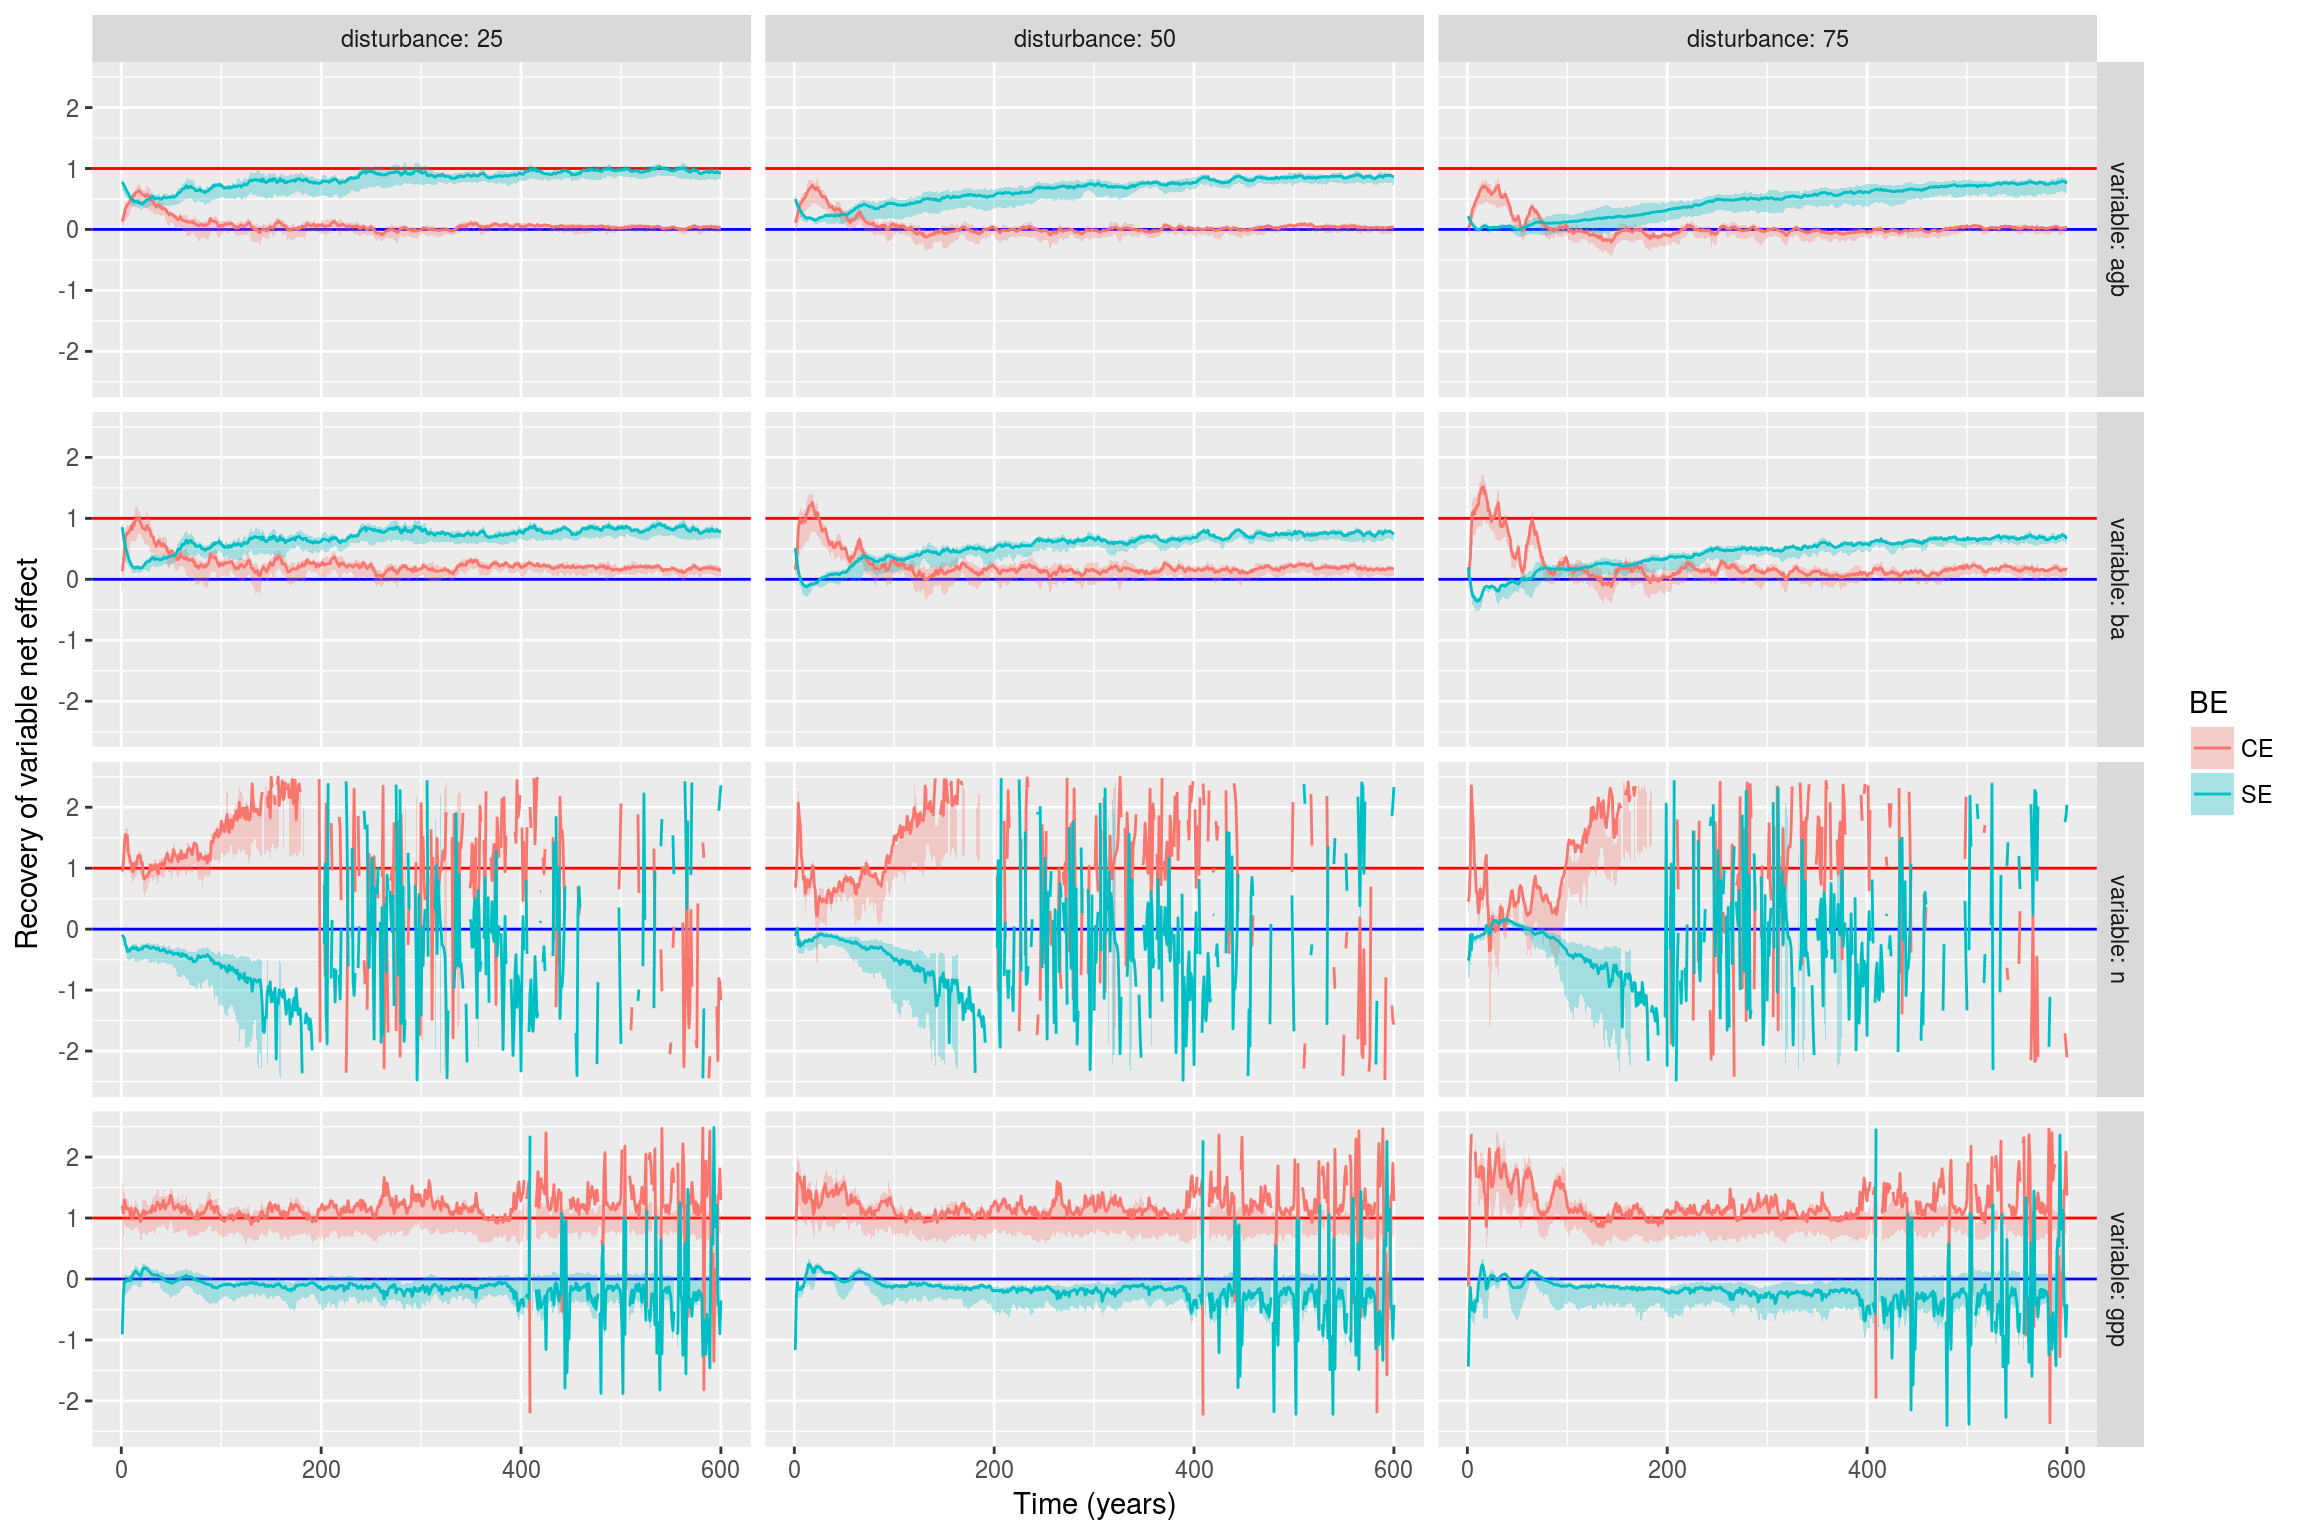
\includegraphics{master-thesis_files/figure-latex/A5allBE-1.pdf}
\caption{\label{fig:A5allBE}Resilience of complementarity and selection
effects. Complementarity effect (CE) and selection effect (SE) where
normalized by control net effect (NEc), thus measuring their resilience
over time for different ecosystem variables (AGB, BA, N, GPP).}
\end{figure}

\addcontentsline{toc}{section}{References}
\bibliography{/home/sylvain/Documents/Bibliography/library.bib}
\listoftables
\listoffigures

% Last pages
  %Last page
  \newpage
  \paragraph{Résumé :}
  Écrire le résumé ici...
  \paragraph{Mots clés :} mots clés
  \newline\newline
  \paragraph{Abstract:}
  Write abstract here
  \paragraph{Keywords:} keywords
  
  \vspace*{\fill}
  
\includegraphics{images/logo}

\end{document}
